%This is a LaTeX template for homework assignments
\documentclass{article}
\usepackage[utf8]{inputenc}
\usepackage{graphicx}
\usepackage{amsmath,amsfonts,amssymb}

\def\tf{\textbf}
\def\tt{\textit}
\def\mc{\ensuremath\mathcal}
\def\mf{\ensuremath\mathbf}
\def\mt{\ensuremath\mathit}
\def\mb{\ensuremath\mathbb}
\def\td{\ensuremath\tilde}
\def\N{\ensuremath\mb{N}}
\def\Z{\ensuremath\mb{Z}}
\def\C{\ensuremath\mb{C}}
\def\R{\ensuremath\mb{R}}
\def\S{\ensuremath\mb{S}}
\def\Ber{\ensuremath\mf{Ber}}
\def\det{\ensuremath\mf{det}}
\def\sigm{\ensuremath\mf{sigm}}
\def\diag{\ensuremath\mf{diag}}
\def\dom{\ensuremath\mf{dom}}
\def\cond{\ensuremath\mf{cond}}
\def\sign{\ensuremath\mf{sign}}
\def\bd{\ensuremath\mf{bd}}
\def\Im{\ensuremath\mf{Im}}
\def\rto{\ensuremath\rightarrow\ }
\def\Rto{\ensuremath\Rightarrow\ }
\def\lto{\ensuremath\leftarrow\ }
\def\Lto{\ensuremath\Leftarrow\ }
\def\xrto{\ensuremath\xrightarrow}
\def\xRto{\ensuremath\xRightarrow}
\def\xlto{\ensuremath\xleftarrow}
\def\xLto{\ensuremath\xLeftarrow}
\def\rvec{\ensuremath\overrightarrow}
\def\lvec{\ensuremath\overleftarrow}

\providecommand\P[1]{}
\renewcommand\P[1]{\mb{P}\{#1\}}
\providecommand\E[1]{}
\renewcommand\E[1]{\mb{E}[#1]}
\providecommand\Var[1]{}
\renewcommand\Var[1]{\mf{Var}(#1)}
\providecommand\p[2]{}
\renewcommand\p[2]{\frac{\partial #1}{\partial #2}}
\providecommand\pp[2]{}
\renewcommand\pp[2]{\frac{\partial^2 #1}{\partial #2^2}}
\providecommand\ps[3]{}
\renewcommand\ps[3]{\frac{\partial^2 #1}{\partial #2\partial #3}}
\providecommand\d[2]{}
\renewcommand\d[2]{\frac{d #1}{d #2}}

\DeclareMathOperator{\sech}{sech}
\DeclareMathOperator{\csch}{csch}

\newcounter{exno}
\setcounter{exno}{1}

\begin{document}
\raggedright

\begin{center}
    \textbf{\Large{Solution Manual}}\\~\\
    \textit{prepared by}\\~\\
    Dhruv Kohli\\~\\
    \textit{for}\\~\\
    \textbf{\Large{Visual Complex Analysis}}\\~\\
    \textit{by}\\~\\
    \large{Tristan Needham}~\\
\end{center}
\clearpage

\begin{center}
    \textbf{\large{1. Geometry and Complex Arithmetic}}
\end{center}

${\textbf{Ex. 1.\theexno}}$
\addtocounter{exno}{1}

\tf{(i)} Inflection point at $f''(X)=0$.\\~\\

\tf{(ii)} [1.1 (ii) TODO]\\~\\

\tf{(iii)} Replacing $X=x-A/3$ we get,

\begin{align*}
    Y &= (x-A/3)^3 + A(x-A/3)^2 + B(x-A/3) + C\\
    &= x^3 - Ax^2 -A^2x/3 -A^3/27 + Ax^2 - 2xA^2/3 +A^3/9 + Bx - AB/3 + C\\
    &= x^3 +(B-A^2)x +2A^3/27-AB/3+C
\end{align*}

\vspace{0.2in}
%%%%%%%%%%%%%%%%%%%%%%%%%%%%%%%%%

${\textbf{Ex. 1.\theexno}}$
\addtocounter{exno}{1}

\tf{(i)} 

\begin{align*}
    (s+t)^3 &= 2p(s+t) + 2q\\
    s^3 + t^3 + 3s^2t + 3st^2 &= 2ps + 2pt + 2q\\
\end{align*}

If $st=p$ and $s^3+t^3=2q$ then above equation satisfies.\\~\\

\tf{(ii)} Put $t=p/s$ in second equation to get,

\begin{align*}
    s^3 + p^3/s^3 &= 2q\\
    (s^3)^2 + p^3 &= 2qs^3
\end{align*}

\tf{(iii)} Solving above quadratic in $s^3$, we get,

\begin{align*}
    s^3 &= \frac{2q \pm \sqrt{4q^2 - 4p^3}}{2}\\
    &= q \pm \sqrt{q^2-p^3}
\end{align*}

By symmetry, $t^3 = 2q-s^3 = q \mp \sqrt{q^2-p^3}$.\\~\\

\tf{(iv)} 

\begin{align*}
    x &= s+t\\
    &= (q + \sqrt{q^2-p^3})^{1/3} + (q - \sqrt{q^2-p^3})^{1/3} 
\end{align*}

\vspace{0.2in}
%%%%%%%%%%%%%%%%%%%%%%%%%%%%%%%%%

${\textbf{Ex. 1.\theexno}}$
\addtocounter{exno}{1}

\tf{(i)}

\begin{align*}
    (2\sqrt{p}C)^3 &= 3p(2\sqrt{p}C) + 2q\\
    8p\sqrt{p}C^3 &= 6p\sqrt{p}C + 2q\\
    4C^3 - 3C &= q/(p\sqrt{p})
\end{align*}

\tf{(ii)} $q/(p\sqrt{p}) \in [-1,1]$. So,

\begin{align*}
    \cos 3\theta &= q/(p\sqrt{p})\\
    \theta &= \frac{1}{3}(\cos^{-1}(q/(p\sqrt{p})) + 2m\pi)\\
    x &= 2\sqrt{p}C = 2\sqrt{p}\cos\left\{\frac{1}{3}(\phi + 2m\pi \right\}
\end{align*}

\tf{(iii)} $p=1, q=0$. Then, $\phi = \pi/2, 3\pi/2$. For all integer values of $m$ and $\sqrt{p}=1$, we have $x=\sqrt{3}, 0$ and $\sqrt{p}=-1$, we have $x=-\sqrt{3},0$.

\vspace{0.2in}
%%%%%%%%%%%%%%%%%%%%%%%%%%%%%%%%%

${\textbf{Ex. 1.\theexno}}$
\addtocounter{exno}{1}

Let $z_1=a+ib$ and $z_2=c+id$. Then, $M=|z_1|^2$ and $N=|z_2|^2$. Then, $MN = |z_1z_2|^2 = (ac-bd)^2 + (ad+bc)^2$.

\vspace{0.2in}
%%%%%%%%%%%%%%%%%%%%%%%%%%%%%%%%%

${\textbf{Ex. 1.\theexno}}$
\addtocounter{exno}{1}

Construct a traiangle $obp$ similar to $o1a$ by drawing straight line originating form $o$ making an angle $\angle ao1$ with $ob$, and by drawing a straight line originating from $b$ making an angle $o1a$ with $ob$. Mark the point of intersection of two lines as $p$. Since the two triangles are similar (by $AA$ similarity), $|p|/|a| = |b|/1$ i.e. $|p|=|a||b|$, and $\arg p = \arg a + \arg b$. Therefore,  $p = ab$.

\vspace{0.2in}
%%%%%%%%%%%%%%%%%%%%%%%%%%%%%%%%%

${\textbf{Ex. 1.\theexno}}$
\addtocounter{exno}{1}

\tf{(i)} Distance of $z$ from $c$ is a fixed number $R$. The locus of $z$ thus, can only be a circle. Algebraically, let $z=x+iy$, then $(x-c_x)^2+(y-c_y)^2 = R^2$ which is equation of a circle.\\~\\

\tf{(ii)} Since, $|3-4i|=5>2$, minimum and maximum value of $|z|$ will be $|3-4i|-2$ and $|3-4i|+2$. These values belong to points at the intersection of circle and the line through origin and centre of circle i.e. $((3-4i)/|3-4i|)(|3-4i|-2)$ and $((3-4i)/|3-4i|)(|3-4i|+2)$.

\vspace{0.2in}
%%%%%%%%%%%%%%%%%%%%%%%%%%%%%%%%%

${\textbf{Ex. 1.\theexno}}$
\addtocounter{exno}{1}

Distance from $a$ is equal to distance from $b$. Thus locus is a line passing through $(a+b)/2$ and perpendicular to $b-a$.

\vspace{0.2in}
%%%%%%%%%%%%%%%%%%%%%%%%%%%%%%%%%

${\textbf{Ex. 1.\theexno}}$
\addtocounter{exno}{1}

$e^{-i\phi}$ rotates the line so that the resulting line is horizontal intersecting imaginary axis at $id$ or $-id$. Algebraically, equation of line is, $z(t) = de^{-i(\pi/2-\phi)} +te^{i\phi}$ so that $e^{-i\phi}z(t) = de^{-i\pi/2}+t = -id + t$.

\vspace{0.2in}
%%%%%%%%%%%%%%%%%%%%%%%%%%%%%%%%%

${\textbf{Ex. 1.\theexno}}$
\addtocounter{exno}{1}

[1.9 TODO]

\vspace{0.2in}
%%%%%%%%%%%%%%%%%%%%%%%%%%%%%%%%%

${\textbf{Ex. 1.\theexno}}$
\addtocounter{exno}{1}

\begin{figure}[h!]
    \centering
    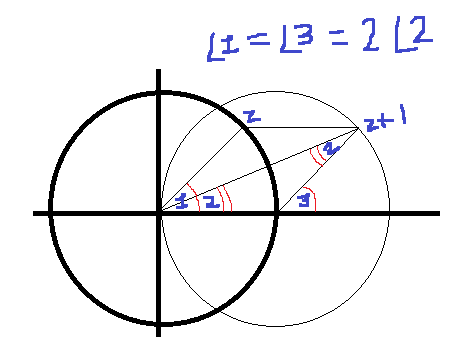
\includegraphics[scale=0.85]{1_10}
    \label{1_10}
\end{figure}

\begin{align*}
    \frac{z}{(z+1)^2} &= \frac{\bar{z}}{(\bar{z}+1)^2}\\
    z(\bar{z}+1)^2 &= \bar{z}(z+1)^2\\
    z\bar{z}^2 + 2|z|^2 + z &= \bar{z}z^2 + 2|z|^2 + \bar{z}\\
    (\bar{z}-z)(|z|^2 - 1) &= 0\\
\end{align*}

So, points on the real axis also satisfy the condition.

\vspace{0.2in}
%%%%%%%%%%%%%%%%%%%%%%%%%%%%%%%%%

${\textbf{Ex. 1.\theexno}}$
\addtocounter{exno}{1}

Given a circle passing through $a$ and $b$, chord $ab$ subtends same angle $\theta$ and $\pi-\theta$ at all points on the two arcs of the circle respectively. Taking a point $z$ on first arc we see that $\arg((z-a)/(z-b)) = \theta$ or $-\theta$. Given the value of constant $c$ in the question, the locus will thus be an arc of a certain circle.

\vspace{0.2in}
%%%%%%%%%%%%%%%%%%%%%%%%%%%%%%%%%

${\textbf{Ex. 1.\theexno}}$
\addtocounter{exno}{1}

\begin{align*}
    \arg\left(\frac{z-1-i}{z+1+i}\right) = \pm \pi/2
\end{align*}

This is a circle passing through $1+i$ and $-1-i$ s.t. the two points are diameterically opposite.

\begin{align*}
    \arg\left(\frac{z-1-i}{z+1+i}\right) = 0, \pi
\end{align*}

This is a straight line (circle of infinite radius) passing through $1+i$ and $-1-i$.

\vspace{0.2in}
%%%%%%%%%%%%%%%%%%%%%%%%%%%%%%%%%

${\textbf{Ex. 1.\theexno}}$
\addtocounter{exno}{1}

\begin{align*}
    \arg \left(\frac{a-b}{a-c}\right) &= \arg\left(\frac{c-a}{c-b}\right) = k
\end{align*}

So, $a$ lies on arc of a certain circle passing through $b$ and $c$. ALso, $c$ lies on arc of a certain circle passing through $a$ and $b$. So, $a$, $b$ and $c$ lie on a circle and form a triangle.

\begin{align*}
    |b-a||b-c| = |a-c|^2
\end{align*}

So, sides of the triangle $bca$ i.e. $bc$, $ca$, $ab$ are in geometric progression.

\vspace{0.2in}
%%%%%%%%%%%%%%%%%%%%%%%%%%%%%%%%%

${\textbf{Ex. 1.\theexno}}$
\addtocounter{exno}{1}

Let $2+i = r_1e^{i\theta_1}$ where $r_1=\sqrt{5}$ and $\theta_1 = \tan^{-1}(1/2)$. Also, let $3+i=r_2e^{i\theta_2}$ where $r_2 = \sqrt{10}$ and $\theta_2 = \tan^{-1}(1/3)$. Since $(2+i)(3+i) = 5 + 5i$ which is also equal to $r_1r_2e^{i\theta_1+\theta_2}$, therefore, $\theta_1+\theta_2 = \tan^{-1}(5/5) = \tan^{-1}(1)=\pi/4$.

\vspace{0.2in}
%%%%%%%%%%%%%%%%%%%%%%%%%%%%%%%%%

${\textbf{Ex. 1.\theexno}}$
\addtocounter{exno}{1}

$e^{i\pi/4} = 1/\sqrt{2}+i/\sqrt{2}$ and $e^{i\pi/2} = i$ and their sum if $e^{i\pi/4}+e^{i\pi/2} = 1/\sqrt{2}+i(1+1/\sqrt{2})$. If one draws the two complex numbers, since their lengths are $1$, their sum will bisect the two numbers and will have argument of $3\pi/8$. So, $\tan(3\pi/8) = \sqrt{2}+1$.

\vspace{0.2in}
%%%%%%%%%%%%%%%%%%%%%%%%%%%%%%%%%

${\textbf{Ex. 1.\theexno}}$
\addtocounter{exno}{1}

Sequence is $1, 1+i, 1+i + i/2\cdot i, 1+i+i/2\cdot i+ i/2\cdot i \cdot i/3, \ldots$. The $n+1$th term will be, $\sum_{k=0}^{n}i^{k}/k!$ which as $n\rto \infty$ approaches $e^{i} = \cos 1 + i\sin 1$.

\vspace{0.2in}
%%%%%%%%%%%%%%%%%%%%%%%%%%%%%%%%%

${\textbf{Ex. 1.\theexno}}$
\addtocounter{exno}{1}

\begin{align*}
    (z-1)/(z+1) &= \frac{\cos\theta-1+i\sin\theta}{\cos\theta+1+i\sin\theta}\\
    &= \frac{(\cos\theta)^2 - (i\sin\theta+1)^2}{(\cos\theta+1)^2 + (\sin\theta)^2}\\
    &= \frac{2i\sin\theta}{2+2\cos\theta}\\
    &= \frac{2i\sin\theta/2\cos\theta/2}{2\cos^2\theta/2}\\
    &= i\tan\theta/2
\end{align*}

\vspace{0.2in}
%%%%%%%%%%%%%%%%%%%%%%%%%%%%%%%%%

${\textbf{Ex. 1.\theexno}}$
\addtocounter{exno}{1}

\begin{align*}
    e^{i\theta} + e^{i\phi} &= (\cos\theta + \cos\phi) + i(\sin\theta + \sin\phi)\\
    &= 2\cos((\theta+\phi)/2)\cos((\theta-\phi)/2) + 2i\sin((\theta+\phi)/2)\cos((\theta-\phi)/2)\\
    &= 2\cos((\theta-\phi)/2)e^{i(\theta+\phi)/2}
\end{align*}

For picture, sum of two vectors results in a vector that bisects angle between the two vectors.

\vspace{0.2in}
%%%%%%%%%%%%%%%%%%%%%%%%%%%%%%%%%

${\textbf{Ex. 1.\theexno}}$
\addtocounter{exno}{1}

[1.19 TODO]
$pca \sim rbc$, $pca \sim qab$ and $rbc \sim qab$ so that,

\begin{align*}
    pc/ca &= rb/bc = qa/ab = k\\
    \angle pca &= \angle qab = \angle rbc = \theta\\
    p-c &= k|c-a|
\end{align*}

\vspace{0.2in}
%%%%%%%%%%%%%%%%%%%%%%%%%%%%%%%%%

${\textbf{Ex. 1.\theexno}}$
\addtocounter{exno}{1}

Suppose $O$ is one vertex, $z=a+ib$ be another vertex s.t $a,b \in \Z$. The third vertex must be $e^{\pm i\pi/3}z = (\sqrt{3}/2+i/2)z$, real part of which is $(\sqrt{3}a-b)/2$ which cannot be integer due to presence of $\sqrt{3}$.

\vspace{0.2in}
%%%%%%%%%%%%%%%%%%%%%%%%%%%%%%%%%

${\textbf{Ex. 1.\theexno}}$
\addtocounter{exno}{1}

$p$ goes to $s$ and $r$ goes to $q$ so that $pr$ goes to $sq$.

\vspace{0.2in}
%%%%%%%%%%%%%%%%%%%%%%%%%%%%%%%%%

${\textbf{Ex. 1.\theexno}}$
\addtocounter{exno}{1}

\begin{align*}
    p &= a-ia\\
    q &= 2a + b -ib\\
    r &= 2a + 2b + c -ic\\
    s &= 2a + 2b + 2c + d -id\\
    A = r-p &= a+ia + 2b + c-ic\\
    B = s-q &= b+ib + 2c + d-id\\
    A+iB &= a+2b+c-b+d + i(a-c+b+2c+d)\\
    &= 0
\end{align*}

So, $B=iA$ and the result still holds.

\vspace{0.2in}
%%%%%%%%%%%%%%%%%%%%%%%%%%%%%%%%%

${\textbf{Ex. 1.\theexno}}$
\addtocounter{exno}{1}

\vspace{0.2in}
%%%%%%%%%%%%%%%%%%%%%%%%%%%%%%%%%

${\textbf{Ex. 1.\theexno}}$
\addtocounter{exno}{1}

\tf{(i)} $z=re^{i\theta}$. For the series to converge $z^{n}$ must converge to $0$. This is possible only when $|z|<1$.\\~\\

\tf{(ii)} Series converges to $1/(1-z)$.\\~\\

\tf{(iii)} $(1+i)/2 = 1/\sqrt{2}e^{i\pi/4}$. $1/(1-z) = 1+i$.

\vspace{0.2in}
%%%%%%%%%%%%%%%%%%%%%%%%%%%%%%%%%

${\textbf{Ex. 1.\theexno}}$
\addtocounter{exno}{1}

\begin{align*}
    S &= \mf{Re}(e^{i\theta}+e^{3i\theta}+e^{5i\theta}+\ldots+e^{(2n-1)\theta})\\
    &= \mf{Re}(e^{i\theta}(1+e^{2i\theta}+e^{4i\theta}+\ldots+e^{(2n-2)\theta}))
    &= \mf{Re}(e^{i\theta}e^{i\theta}(e^{i2n\theta}-1)/(e^{2i\theta}-1))\\
    &= \frac{\sin 2n\theta}{2\sin\theta}
\end{align*}

\vspace{0.2in}
%%%%%%%%%%%%%%%%%%%%%%%%%%%%%%%%%

${\textbf{Ex. 1.\theexno}}$
\addtocounter{exno}{1}

\tf{(i)}

\begin{align*}
    (a+ib)e^{i\theta} &= \sqrt{a^2+b^2}e^{i(\theta + \tan^{-1}(b/a))}\\
    b\cos\theta + a\sin\theta &= \sqrt{a^2+b^2}\sin(\theta+\tan^{-1}(b/a))
\end{align*}

\tf{(ii)}


\vspace{0.2in}
%%%%%%%%%%%%%%%%%%%%%%%%%%%%%%%%%

${\textbf{Ex. 1.\theexno}}$
\addtocounter{exno}{1}

\begin{align*}
    |Z(t)| = r &= e^{at}\\
    \arg Z(t) = \theta &= bt\\
\end{align*}

Eliminate $t$ to get $r(\theta) = e^{(a/b)\theta}$.

\vspace{0.2in}
%%%%%%%%%%%%%%%%%%%%%%%%%%%%%%%%%

${\textbf{Ex. 1.\theexno}}$
\addtocounter{exno}{1}

\tf{(i)}

\begin{align*}
    \mc{F}_{\tau}[Z(t)] &= (e^{a\tau}e^{ib\tau})e^{at}e^{ibt}\\
    &= e^{a(\tau+t)}e^{ib(t+\tau)}\\
    &= Z(t+\tau)
\end{align*}

\vspace{0.2in}
%%%%%%%%%%%%%%%%%%%%%%%%%%%%%%%%%

${\textbf{Ex. 1.\theexno}}$
\addtocounter{exno}{1}

\vspace{0.2in}
%%%%%%%%%%%%%%%%%%%%%%%%%%%%%%%%%

${\textbf{Ex. 1.\theexno}}$
\addtocounter{exno}{1}

\vspace{0.2in}
%%%%%%%%%%%%%%%%%%%%%%%%%%%%%%%%%

${\textbf{Ex. 1.\theexno}}$
\addtocounter{exno}{1}

\vspace{0.2in}
%%%%%%%%%%%%%%%%%%%%%%%%%%%%%%%%%

${\textbf{Ex. 1.\theexno}}$
\addtocounter{exno}{1}

Put $a=e^{i\theta}$ and $b=e^{-i\theta}$ to get

\vspace{0.2in}
%%%%%%%%%%%%%%%%%%%%%%%%%%%%%%%%%

${\textbf{Ex. 1.\theexno}}$
\addtocounter{exno}{1}

\vspace{0.2in}
%%%%%%%%%%%%%%%%%%%%%%%%%%%%%%%%%

${\textbf{Ex. 1.\theexno}}$
\addtocounter{exno}{1}

\vspace{0.2in}
%%%%%%%%%%%%%%%%%%%%%%%%%%%%%%%%%

${\textbf{Ex. 1.\theexno}}$
\addtocounter{exno}{1}

\vspace{0.2in}
%%%%%%%%%%%%%%%%%%%%%%%%%%%%%%%%%

${\textbf{Ex. 1.\theexno}}$
\addtocounter{exno}{1}

\vspace{0.2in}
%%%%%%%%%%%%%%%%%%%%%%%%%%%%%%%%%

${\textbf{Ex. 1.\theexno}}$
\addtocounter{exno}{1}

\tf{(i)} $c-b$ can be obtained by rotating $a-b$ by $\phi/2$ and scaling the result. Similarly, $c-a$ can be obtained by rotating $b-a$ by $-\theta/2$ (i.e. $\theta/2$ clockwise) and scaling the result.\\~\\

\tf{(ii)} 

\begin{align*}
    \frac{c-b}{a-b} &= \frac{(a-b)e^{i\phi}(1-e^{i\theta})}{(a-b)(1-e^{i(\theta+\phi)})}\\
    &= \frac{e^{i\phi}(1-e^{i\theta})}{1-e^{i(\theta+\phi)}}\\
    &= \frac{\sin(\theta/2)}{\sin((\theta+\phi)/2)}e^{i\phi/2}
\end{align*}

\tf{(iii)} Same approach as in $\tf{(ii)}$.

\vspace{0.2in}
%%%%%%%%%%%%%%%%%%%%%%%%%%%%%%%%%

${\textbf{Ex. 1.\theexno}}$
\addtocounter{exno}{1}

\vspace{0.2in}
%%%%%%%%%%%%%%%%%%%%%%%%%%%%%%%%%

${\textbf{Ex. 1.\theexno}}$
\addtocounter{exno}{1}

\begin{align*}
    R_{c}^{\alpha}(z) &= e^{i\alpha}(z-c)+c\\
    &= e^{i\alpha}z +c(1-e^{i\alpha})\\
    &= e^{i\alpha}z + v\\
    \lim_{\alpha\rto 0} R_{c}^{\alpha}(z) &= z+v
\end{align*}

\vspace{0.2in}
%%%%%%%%%%%%%%%%%%%%%%%%%%%%%%%%%

${\textbf{Ex. 1.\theexno}}$
\addtocounter{exno}{1}



\vspace{0.2in}
%%%%%%%%%%%%%%%%%%%%%%%%%%%%%%%%%

${\textbf{Ex. 1.\theexno}}$
\addtocounter{exno}{1}

\vspace{0.2in}
%%%%%%%%%%%%%%%%%%%%%%%%%%%%%%%%%

${\textbf{Ex. 1.\theexno}}$
\addtocounter{exno}{1}

\vspace{0.2in}
%%%%%%%%%%%%%%%%%%%%%%%%%%%%%%%%%

${\textbf{Ex. 1.\theexno}}$
\addtocounter{exno}{1}

\vspace{0.2in}
%%%%%%%%%%%%%%%%%%%%%%%%%%%%%%%%%

${\textbf{Ex. 1.\theexno}}$
\addtocounter{exno}{1}

\vspace{0.2in}
%%%%%%%%%%%%%%%%%%%%%%%%%%%%%%%%%

${\textbf{Ex. 1.\theexno}}$
\addtocounter{exno}{1}

\vspace{0.2in}
%%%%%%%%%%%%%%%%%%%%%%%%%%%%%%%%%

${\textbf{Ex. 1.\theexno}}$
\addtocounter{exno}{1}

\vspace{0.2in}
%%%%%%%%%%%%%%%%%%%%%%%%%%%%%%%%%

\clearpage
\setcounter{exno}{1}

\begin{center}
    \textbf{\large{3. Mobius Transformations and Inversion}}
\end{center}

${\textbf{Ex. 3.\theexno}}$
\addtocounter{exno}{1}

\tf{(i)} $opc \sim oc\td{p}$ so that $[op]/[oc]=[oc]/[o\td{p}]$. Now use $[oc]=R$.\\~\\

\tf{(ii)} $\angle pco = \angle poc = \angle o\td{p}c$ so that $opc \sim oc\td{p}$. So, $[op]/[oc] = [oc]/[o\td{p}]$. Now use $[oc]=R$.\\~\\

\tf{(iii)} [TODO 3.(iii)]

\vspace{0.2in}
%%%%%%%%%%%%%%%%%%%%%%%%%%%%%%%%%

${\textbf{Ex. 3.\theexno}}$
\addtocounter{exno}{1}

$[op] = \sqrt{l^2-r^2\cos^2\phi/2} - r\sin\phi/2$ and $[o\td{p}] = \sqrt{l^2-r^2\cos^2\phi/2} + r\sin\phi/2$ so that $[op][o\td{p}] = l^2-r^2\cos^2\phi/2 - r^2\sin^2\phi/2 = l^2-r^2$.

\vspace{0.2in}
%%%%%%%%%%%%%%%%%%%%%%%%%%%%%%%%%

${\textbf{Ex. 3.\theexno}}$
\addtocounter{exno}{1}

[TODO 3.3]

\vspace{0.2in}
%%%%%%%%%%%%%%%%%%%%%%%%%%%%%%%%%

${\textbf{Ex. 3.\theexno}}$
\addtocounter{exno}{1}

First note that $z \mapsto -z$ on $\C$ is equivalent to rotation of $\Sigma$ of $\pi$ about vertical axis through $0$ and $N$. To obtain the antipodal point $\hat{q}$ of $\hat{p}$ one requires to rotate $\Sigma$ with $\pi$ about vertical axis through $0$ and $N$ and then reflect the result in the equitorial plane. These two transformations in the complex plane amounts to $z\mapsto -z$ and $z \mapsto \mc{I}_C(z)$ (Used (17) to obtain the second transformation).

\vspace{0.2in}
%%%%%%%%%%%%%%%%%%%%%%%%%%%%%%%%%

${\textbf{Ex. 3.\theexno}}$
\addtocounter{exno}{1}

Projecting from $S$ is equivalent to taking reflection of $\Sigma$ in equitorial plane and then projecting from $N$. So, $f(z)=\mc{I}_C(z)$.

\vspace{0.2in}
%%%%%%%%%%%%%%%%%%%%%%%%%%%%%%%%%

${\textbf{Ex. 3.\theexno}}$
\addtocounter{exno}{1}

\tf{(i)} $\angle p0N = \angle N0q = \pi/2$ and $\angle 0Np = \pi/2-\angle Np0 = \pi/2 - \angle qN0$, so, $\angle Np0 = \angle qN0$. So, $[0p]/[0N] = [0N]/[0q]$\\~\\

\tf{(ii)} $\angle N0z = \angle \td{z}0N$. $\theta = \angle N\td{z}0 = \angle z \hat{\td{z}} \hat{z}$, $\angle \hat{z}z\td{z} = \pi/2-\theta$, $\angle Nz0 = \angle \hat{z}z\td{z}$, $\angle 0Nz = \pi/2-\angle Nz0 = \pi/2-(\pi/2-\theta)= \theta$. So, $z0N \sim N0\td{z}$. So, $[0z]/[0N] = [0N]/[0\td{z}]$.

\vspace{0.2in}
%%%%%%%%%%%%%%%%%%%%%%%%%%%%%%%%%

${\textbf{Ex. 3.\theexno}}$
\addtocounter{exno}{1}

[TODO 3.7]

\vspace{0.2in}
%%%%%%%%%%%%%%%%%%%%%%%%%%%%%%%%%

${\textbf{Ex. 3.\theexno}}$
\addtocounter{exno}{1}

Vertical component of velocity is $\cos\phi$ and horizontal component is $\sin\phi$. The collision time $t$ is given by $1+t\cos\phi = t$ so that $t = 1/(1-\cos\phi)$. Clearly, the collision points will be in direction of $e^{i\theta}$. The collision point is at a distance $t\sin\phi$ from the origin, so that associated complex number is $\sin\phi/(1-\cos\phi)e^{i\theta} = \cot(\phi/2)e^{i\theta}$.

\vspace{0.2in}
%%%%%%%%%%%%%%%%%%%%%%%%%%%%%%%%%

${\textbf{Ex. 3.\theexno}}$
\addtocounter{exno}{1}

\tf{(i)} $A = 1\sin\theta + 1\sin\theta$ and $B = 1\sin(\pi/2-\theta) + 1\sin(\pi/2-\theta)$.\\~\\

\tf{(ii)} $[ab][cd] + [ad][bc] = [ac][bd]$ so that $2\sin\phi\cdot 2\cos\theta + 2\cos\phi\cdot 2\sin\phi = 2\sin(\theta+\phi)\cdot 2\sin\pi/2$.

\vspace{0.2in}
%%%%%%%%%%%%%%%%%%%%%%%%%%%%%%%%%

${\textbf{Ex. 3.\theexno}}$
\addtocounter{exno}{1}

\tf{(i)} WLOG let the two circles be $(0,0),1$ and $(x,0),r$ where $x>r+1$ or $0 < x < 1-r$. Clearly the only way two points can be symmetric is when the point lies on $x$ axis and one of them, $(y,0)$, is s.t. $0 < y < 1$ in first case and $x < y < x+r$. In the first case, the symmetric point is $(0,1/y)$ and so $(x-y)(x-1/y) = r^2$ i.e. $x^2-xy-r^2+1 = x/y$. Plotting LHS and RHS separately as a function of $y$, we have RHS at $y=0$ is $\infty$ and at $y=1$ is $x$, and LHS at $y=0$ is $x^2-r^2+1 = (x-r)(x+r)+1 > x+r+1 > x$ and at $y=1$ is $x^2-x-r^2+1 < x^2-x-(x-1)^2+1 = x$ so that there must be one intersection point and one solution. The two symmetric points will then be $(y,0)$ and $(1/y,0)$.\\~\\

\tf{(ii)} $\xi_{\pm}$ are symmetric about $A$ and $B$. Mobius transformation preserves circles and symmetry so $0,\infty$ are symmetric about circles $F(A)$ and $F(B)$ therefore, $F(A)$ and $F(B)$ are concentric centred at origin.

\vspace{0.2in}
%%%%%%%%%%%%%%%%%%%%%%%%%%%%%%%%%

${\textbf{Ex. 3.\theexno}}$
\addtocounter{exno}{1}

[TODO 3.11]

\vspace{0.2in}
%%%%%%%%%%%%%%%%%%%%%%%%%%%%%%%%%

${\textbf{Ex. 3.\theexno}}$
\addtocounter{exno}{1}

First note that given two concentric circles, if one choice of $C_1$ closes the chain then all choices of $C_1$ will close the chain. Now, Given two non-concentric non-intersecting circles $A$ and $B$ as in the figure in question, suppose for a choice of $C_1$, the chain closes. Consider the M.T. described in \tf{Ex. 3.10}, then $A$ and $B$ will map to concentric circles centred at origin, while $C_1$ and all other circles in chain maps to equal radius circles sandwiched the two concentric circles. Since each circle in chain touches $A$ and $B$ and the adjacent circles, same will be true for the mapped chain. Since the original chain closes, so the mapped chain closes too. Now, take an arbitrary $C_1$ and the chain generated from it. They will map to a circle sandwiched between the two concentric circles and the chain generated from it. Since the later will always close because of the argument in first line, the former will close too.

\vspace{0.2in}
%%%%%%%%%%%%%%%%%%%%%%%%%%%%%%%%%

${\textbf{Ex. 3.\theexno}}$
\addtocounter{exno}{1}

\tf{(i)} Easy to see that the angle subtended by a circle in chain is $2\sin^{-1}(1/2) = \pi/3$ so that the chain will comprise of $2\pi/(\pi/3) = 6$ circles.\\~\\

\tf{(iii)} Applying Inversion in a circle centred at the intersection point of $A$ and $B$, $\td{A}$ and $\td{B}$ will be two parallel planes and $\td{C}$ will be a sphere sandwiched between the two planes. The chain of spheres in the chain will map to the chain of spheres sandwiched between the two planes touching one another successively and touching $\td{C}$. Using $\tf{(i)}$ we conclude that the chain closes with the six spheres.

\vspace{0.2in}
%%%%%%%%%%%%%%%%%%%%%%%%%%%%%%%%%

${\textbf{Ex. 3.\theexno}}$
\addtocounter{exno}{1}

Using the fact that area of a triangle is given by $0.5 \times $ base $\times$ height and is also given by $0.5 ab \sin C$. Note that height of each triangle is same. Let it be $h$.

\begin{align*}
    [a,b,c,d] &= \frac{(a-b)(c-d)}{(c-b)(a-d)}\\
    &= -\frac{\Delta_{\alpha}\Delta_{\gamma}}{\Delta_{\beta}\Delta_{\delta}}\\
    &= -\frac{[oa][ob]\sin\alpha [oc][od]\sin\gamma}{[ob][oc]\sin\beta [oa][od]\sin\delta}
\end{align*}

Angles subtended at the eye remain same.

\vspace{0.2in}
%%%%%%%%%%%%%%%%%%%%%%%%%%%%%%%%%

${\textbf{Ex. 3.\theexno}}$
\addtocounter{exno}{1}

$Arg [z,q,r,s] = Arg(((z-q)(r-s))/((z-s)(r-q)))$. $q-z = k_1e^{i\theta}(s-z)$ and $s-r = k_2e^{i\phi}(s-r)$.\\~\\

$q-z = k_3e^{i\theta}(s-z)$ and $(s-r)=k_4e^{i\phi} (q-r)$.

If $p,q,r,s$ lie on circle passing through $q,r,s$, then $\theta+\phi=\pi$ and result follows.

\vspace{0.2in}
%%%%%%%%%%%%%%%%%%%%%%%%%%%%%%%%%

${\textbf{Ex. 3.\theexno}}$
\addtocounter{exno}{1}

\tf{(i)} $q,r,s$ are mapped to $0,1\infty$, $1,0,\infty$ and so on. Recall that M.T. is uniquely determined by the images of three fixed points in $\C$.

\tf{(ii)} $[z,q,r,s]$ sends $q$ to $0$, $r$ to $1$ and $s$ to $\infty$. If $I$ swaps $0$ with $\infty$ then $I \circ [z,q,r,s]$ will send $q$ to $\infty$, $r$ to $1$ and $s$ to $0$. By uniqueness theorem, the resulting M.T. will be $[z,s,r,q]$.\\~\\

\tf{(iii)} Same approach as \tf{(ii)}.\\~\\

\tf{(iv)} Image of $(q,r,s)$ with: $\chi$ is $(0,1,\infty)$, with $I\circ \chi$ is $(\infty,1,0)$, with $J \circ \chi$ is $(1,\infty,0)$, with $I\circ J\circ \chi$ is $(1,0,\infty)$, with $J\circ I \circ \chi$ is $(0,\infty,1)$ and with $I\circ J \circ I \circ \chi$ is $(\infty,0,1)$.\\~\\

\tf{(v)} Can be done algebraically using \tf{(ii)} and \tf{(iii)}. Can be done directly too.\\~\\

\tf{(vi)} Using \tf{(iv)} and \tf{(v)}.

\vspace{0.2in}
%%%%%%%%%%%%%%%%%%%%%%%%%%%%%%%%%

${\textbf{Ex. 3.\theexno}}$
\addtocounter{exno}{1}

Image of $K$ will be a circle $K'$ passing through image of $c$ which is $1+0i$ s.t. images of $b$ and $d$ which are $0$ and $\infty$ respectively, are symmetric wrt to $K'$. So, the centre of $K'$ must be $0$ and its radius must be $1$. Since M.T. preserves circle, image of $a$ lies on $K'$.

\vspace{0.2in}
%%%%%%%%%%%%%%%%%%%%%%%%%%%%%%%%%

${\textbf{Ex. 3.\theexno}}$
\addtocounter{exno}{1}

Translation of $d/c$ shifts real axis to horizontal line at height $\mf{Im}(d/c)$. Then, complex inversion in unit circle results in a circle through origin, with diameter $1/|\mf{Im}(d/c)|$. Then, dilative rotation about origin of $-(ad-bc)/c^2 = -1/c^2$ (because $M(z)$ is normalized) makes the radius $1/|2c^2\mf{Im}(d/c)|$ and shifts centre of circle (but the circle still passes through origin). Then, another translation shifts the origin to $a/c$ and does not change the radius.

\vspace{0.2in}
%%%%%%%%%%%%%%%%%%%%%%%%%%%%%%%%%

${\textbf{Ex. 3.\theexno}}$
\addtocounter{exno}{1}

\tf{(i)} Translation of $d/c$ only shifts the centre of the concentric circles. Then, complex inversion will result in a family of circles which may or may not be concentric [for example consider two concentric circles such that the outer circle intersects the unit circle at right angles then with complex inversion the centre of the two circles will change]. Then, dilative rotation about origin will change the radius and shift centre of resulting circles. Finally, another translation again shifts centre of resulting circles.\\~\\

\tf{(ii)} If after geometric inversion (a part of complex inversion), the circles have same centre then they will stay concentric. Geometric inversion results in concentric circles if and only if the original circles are concentric with origin as centre. Since the first step of M.T. is to translate by $d/c$, therefore, image is concentric circles if and only if the centre of concentric circles is $-d/c$. After complex inversion, centre is $0$. Then after dilative rotation about origin it stays the same. Then translation of $a/c$ shifts centre to $a/c$.\\~\\

\tf{(iii)} $I_M$ is circle centred at $-d/c$ of radius $1/|c|$. Final centre will be $a/c$ and radius will transform as follows $1/|c| \rto 1/|c| \rto |c| \rto |c|/|c|^2 =1/|c| \rto 1/|c|$. Suppose arc subtends $\theta$ at centre, then angle transforms as $\theta \rto \theta \rto \theta \rto \theta \rto \theta$. Since angle subtended and radius is same, size of image arc is same.

\vspace{0.2in}
%%%%%%%%%%%%%%%%%%%%%%%%%%%%%%%%%

${\textbf{Ex. 3.\theexno}}$
\addtocounter{exno}{1}

\tf{(i)} $a$ and $\theta$ be s.t. $q/p = a$ and $p = e^{i(\pi+\theta/2)}$. So, $M(z) = p(z+q/p)/(-\bar{p}(-(\bar{q}/\bar{p})z-1)) = e^{i\theta}(z-a)/(\bar{a}z-1)$.\\~\\

\tf{(ii)} $[M] = [p,q;\bar{q},\bar{p}]$. $M^{-1} = 1/(|p|^2-|q|^2)[\bar{p},-q;-\bar{q},p]$ which has same form. $[1,0;0,1]$ also has same form. $[M_1][M_2] = [p_1p_2 + q_1\bar{q_2}, p_1q_2 + q_1\bar{p_2}; \bar{q_1}p_2 + \bar{p_1}\bar{q_1}, \bar{q_1}q_2 + \bar{p_1}\bar{p_1}]$ has same form.\\~\\

\tf{(iii)} $M(z) = R^{\theta} \circ M_a$. $M^{-1}(z) = M_a \circ R^{-\theta} = R^{-\theta} \circ M_a$ which has same form. $M_{a_1} \circ M_{a_2} = (a_1\bar{a_2}-1)/(1-\bar{a_1}a_2)(z-(a_1-a_2)/(1-\bar{a_1}a_2))/((\bar{a_1}-\bar{a_2})/(1-a_1\bar{a_2})z - 1)$. Composition of two automorphism is an automorphism. Inverse of automorphism is automorphism and Identity belongs to automorphism.

\vspace{0.2in}
%%%%%%%%%%%%%%%%%%%%%%%%%%%%%%%%%

${\textbf{Ex. 3.\theexno}}$
\addtocounter{exno}{1}

\tf{(i)} Same approach as in previous exercise.\\~\\

\tf{(ii)} If $[R_1]$ and $[R_2]$ preserve inner product then so will $[R_1][R_2]$. $[R_1]^{-1}$ and identity matrix also preserves inner product.

\vspace{0.2in}
%%%%%%%%%%%%%%%%%%%%%%%%%%%%%%%%%

${\textbf{Ex. 3.\theexno}}$
\addtocounter{exno}{1}

$w = x^2-y^2 + 2xyi$. Circle with centre $(1/2,0)$ and radius $1/2$. [TODO 3.22]

\vspace{0.2in}
%%%%%%%%%%%%%%%%%%%%%%%%%%%%%%%%%

${\textbf{Ex. 3.\theexno}}$
\addtocounter{exno}{1}

Complex inversion is composition of $\mc{I}_C$ and $R_{L}$ where $L$ is real axis. Since, unit circle and real axis intersect at two distinct points so complex inversion is elliptic. The angle of intersection is $\pi/2$ so multiplier is $e^{i2(\pi/2)} = -1$.

\vspace{0.2in}
%%%%%%%%%%%%%%%%%%%%%%%%%%%%%%%%%

${\textbf{Ex. 3.\theexno}}$
\addtocounter{exno}{1}

\tf{(i)} Let $a$ be in the upper half-plane which is mapped to $0$. Since $a$ and $\bar{a}$ are symmetric wrt to real axis, $a$ and $1/\bar{a}$ must be symmetric wrt to unit circle so that $1/\bar{a}$ is mapped to $\infty$. So, $M(z) = k(z-a)/(z-\bar{a})$. Let $1$ is mapped to $p$ on the unit circle. So, $|M(1)| = 1 = |k|$. So, $k = e^{i\theta}$ for some $\theta$ where choice of $\theta$ depends on choice of $p$.\\~\\

\tf{(ii)} $[M] = [e^{i\theta},-ae^{i\theta};1,-\bar{a}]$ $[M]^{-1} = 1/(e^{i\theta}(a-\bar{a}))[-\bar{a},ae^{i\theta};-1,e^{i\theta}]$ so that $N(z) = (-\bar{a}z+ae^{i\theta})/(-z+e^{i\theta})$\\~\\

\tf{(iii)} $z$ and $1/\bar{z}$ are symmetric wrt to unit circle. So, their image in $N$ must also be symmetric about real axis. So, $N(1/\bar{z}) = \bar{N(z)}$.\\~\\

\tf{(iv)} Easy.

\vspace{0.2in}
%%%%%%%%%%%%%%%%%%%%%%%%%%%%%%%%%

${\textbf{Ex. 3.\theexno}}$
\addtocounter{exno}{1}

\tf{(i)} Let $q,r,s$ maps to $0,1,\infty$. Then, $M(z) = \frac{(z-q)(r-s)}{(z-s)(r-q)}$. Since $q,r,s$ are real, all coefficients are real.\\~\\

\tf{(ii)} $\mf{Im}[M(i)] > 0$ so, $M(i) = \frac{ai+b}{ci+d} = \frac{i(ad-bc)+db+ac}{c^2+d^2}$.\\~\\

\tf{(iii)} Geometrically, Identity belongs to group, composition of two such automorphism is another automorphism (mapping from upper half plane to upper half plane) and if $M$ sends $q,r,s$ on real axis to $0,1,\infty$ then $M^{-1}$ sends $0,1,\infty$ back to $q,r,s$ and the rest of upper half plane to upper half plane. Algebraically, easy.\\~\\

\tf{(iv)} $3$ degrees of freedom. Geometrically, three real numbers representing points on real axis that map to $0,1,\infty$ are required. Algebraically, $M(z) = (az+b)/(cz+d) = (a/b z + 1)/(c/bz+d/b) = (uz+1)/(vz+w)$ where $u,v,w$ are real.

\vspace{0.2in}
%%%%%%%%%%%%%%%%%%%%%%%%%%%%%%%%%

${\textbf{Ex. 3.\theexno}}$
\addtocounter{exno}{1}

\tf{(i)} $M_a(z) = (z-a)/(\bar{a}z-1)$. Normalized form is $(z/\sqrt{|a|^2-1}-a/\sqrt{|a|^2-1})/(\bar{a}z/\sqrt{|a|^2-1}-1/\sqrt{|a|^2-1})$. So, $a+d = 0$ which is real and $<2$. So, elliptic.\\~\\

\tf{(ii)} $sqrt{m}+1/\sqrt{m}=0$ so that $m = -1$.\\~\\

\tf{(iii)} $[M_a][M_a] = 1/\sqrt{|a|^2-1}[1,-a;\bar{a},-1]1/\sqrt{|a|^2-1}[1,-a;\bar{a},-1] = 1/(1-|a|^2)[1-|a|^2,0;0,1-|a|^2] = I$.\\~\\

\tf{(iv)} Fixed points are $\frac{2/\sqrt{|a|^2-1} \pm 2i}{2\bar{a}/\sqrt{|a|^2-1}} = (1 \pm \sqrt{1-|a|^2})/\bar{a}$\\~\\

\tf{(v)} Radius of $J$ is $\sqrt{|q||a-q|} = \sqrt{(1-|a|^2)}/|a|$ so that $\xi_{\pm} = (R\mp|q|)|a|/\bar{a} = (1+\sqrt{1\mp|a|^2})/\bar{a}$

\vspace{0.2in}
%%%%%%%%%%%%%%%%%%%%%%%%%%%%%%%%%

${\textbf{Ex. 3.\theexno}}$
\addtocounter{exno}{1}

$M_{a}^{\phi} = e^{i\phi}(z-a)/(\bar{a}z-1)$. Normalized form is $\frac{e^{i\phi/2}z/(\sqrt{|a|^2-1}) - e^{i\phi/2}a/(\sqrt{|a|^2-1})}{\bar{a}z/(e^{i\phi/2}\sqrt{|a|^2-1}) - 1/(e^{i\phi/2}\sqrt{|a|^2-1})}$

\tf{(i)} $a+d = -2\sin(\phi/2)/\sqrt{1-|a|^2} = -2\sqrt{1-\cos^2(\phi/2)}/\sqrt{1-|a|^2}$. When $|\phi|<\Phi$, $\cos(\phi/2) > \cos(\Phi/2) = |a|$ so that $(1-\cos^2(\phi/2)) < (1-|a|^2)$. So, $a+d$ is real and $|a+d| < 2$, thus, elliptic.\\~\\

\tf{(ii)} $|\phi| = \Phi$ so that $(1-\cos^2(\phi/2)) = (1-|a|^2)$ and $a+d = \pm -2$, so hyperbolic.\\~\\

\tf{(iii)} $|\phi|>\Phi$ then $(a+d)$ is real and $|a+d|>2$.

\vspace{0.2in}
%%%%%%%%%%%%%%%%%%%%%%%%%%%%%%%%%

\clearpage
\setcounter{exno}{1}

\begin{center}
    \textbf{\large{6. Non-Euclidean Geometry}}
\end{center}

${\textbf{Ex. 6.\theexno}}$
\addtocounter{exno}{1}

$E(\Delta) = a+b+c-\pi$, $E(\Delta_1) = a_1+b+p-\pi$ and $E(\Delta_2) = a_2+c+q-\pi$. Use $p+q = \pi$ and $a_1+a_2 = a$.\\~\\

$E(\Delta) = \lim_{n\rto\infty}\sum_{i=1}^{n} E(\Delta_i) = \lim_{n\rto\infty}\sum_{i=1}^{n}k(p_i)A(\Delta_i) = \int\int k(p)dA$.

\vspace{0.2in}
%%%%%%%%%%%%%%%%%%%%%%%%%%%%%%%%%

${\textbf{Ex. 6.\theexno}}$
\addtocounter{exno}{1}

[TODO 6.2]

\vspace{0.2in}
%%%%%%%%%%%%%%%%%%%%%%%%%%%%%%%%%

${\textbf{Ex. 6.\theexno}}$
\addtocounter{exno}{1}

[TODO 6.3]

\vspace{0.2in}
%%%%%%%%%%%%%%%%%%%%%%%%%%%%%%%%%

${\textbf{Ex. 6.\theexno}}$
\addtocounter{exno}{1}

$(w-\xi_{+})/(w-\xi_{-}) = m(z-\xi_{+})/(z-\xi_{-})$ In matrix notation we have, $[1,-\xi_{+};1,-\xi_{-}][w;1] = [\sqrt{m},-\sqrt{m}\xi_{+};1/\sqrt{m},-\xi_{i}/\sqrt{m}] = [\sqrt{m},0;0,1/\sqrt{m}][1,-\xi_{+};1,-\xi_{-}]$. Now take $\xi_+ = a, \xi_{-} = -1/\bar{a}$ and $m=e^{-i\psi}$ to get,

$[M] = 1/(a+1/\bar{a})[1/\bar{a},a;-1,1][e^{-i\psi/2},0;0,e^{i\psi/2}][1,-a;1,1/\bar{a}]$. Multiply out to get the result.

\vspace{0.2in}
%%%%%%%%%%%%%%%%%%%%%%%%%%%%%%%%%

${\textbf{Ex. 6.\theexno}}$
\addtocounter{exno}{1}

$M'(z) = a(-\bar{b}z+\bar{a})+\bar{b}(az+b))/(-\bar{b}z+\bar{a})^2 = (|a|^2+|b|^2)/(-\bar{b}z+\bar{a})^2$. $(1+|M(z)|^2)/(1+|z|^2) = (((-\bar{b}z+\bar{a})(-b\bar{z}+a) + (az+b)(\bar{a}\bar{z}+\bar{b}))/|(-\bar{b}z+\bar{a})|^2)/(1+|z|^2) = (|a|^2+|b|^2)/(|-\bar{b}z+\bar{a}|^2)$.

\vspace{0.2in}
%%%%%%%%%%%%%%%%%%%%%%%%%%%%%%%%%

${\textbf{Ex. 6.\theexno}}$
\addtocounter{exno}{1}

[TODO 6.6]

\vspace{0.2in}
%%%%%%%%%%%%%%%%%%%%%%%%%%%%%%%%%

${\textbf{Ex. 6.\theexno}}$
\addtocounter{exno}{1}

[TODO 6.7]

\vspace{0.2in}
%%%%%%%%%%%%%%%%%%%%%%%%%%%%%%%%%

${\textbf{Ex. 6.\theexno}}$
\addtocounter{exno}{1}

[TODO 6.8]

\vspace{0.2in}
%%%%%%%%%%%%%%%%%%%%%%%%%%%%%%%%%

${\textbf{Ex. 6.\theexno}}$
\addtocounter{exno}{1}

\tf{(i)} Stereographic projection is conformal. So, the image semi-circle will be orthogonal to the plane. Now projecting this semicircle on the plane results in a straight line connecting the two end points on the plane.\\~\\

\tf{(ii)} $Npq \sim z0S$ so that $pq/Nq = 0S/zS$ i.e. $|z'|/a = 1/b$. And, $z0S \sim NqS$ so that $z0/zS = Nq/NS$ i.e. $|z|/b = a/2$. So, $|z'| = a/b = 2|z|/b^2 = 2|z|/(1+|z|^2)$. Also note that $\arg(z')=\arg(z)$.\\~\\

\begin{figure}[h!]
    \centering
    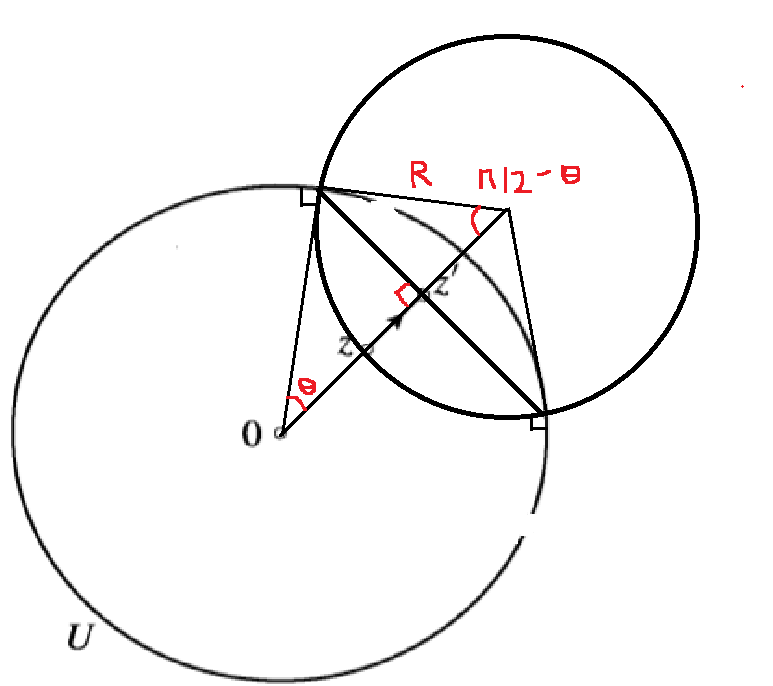
\includegraphics[scale=0.7]{6_9}
    \label{6_9}
\end{figure}

\tf{(iii)} As in the figure, $1-\cos^2\theta = R^2(1-\sin^2\theta)$ so that $R^2 = \tan^2\theta$. Now, $|z'|\sqrt{1+R^2} = |\cos\theta|\sqrt{1+\tan^2\theta} = 1$ so that centre of $C$ is $\mc{I}_U(z')$. Using the fact that orthogonal circles map to themselves under inversion, we have $z$ and $\mc{I}_{U}(z)$ as the opposite ends of a diameter of $C$. So, we have $1/\bar{z'} = (z+1/\bar{z})/2$ so that $z' = 2z/(1+|z|^2)$.

\vspace{0.2in}
%%%%%%%%%%%%%%%%%%%%%%%%%%%%%%%%%

${\textbf{Ex. 6.\theexno}}$
\addtocounter{exno}{1}

Let $(x,\sigma)$ represents a point on the sphere where $x$ represents the angle around the axis (vertical line through centre) where $x\in [0,2\pi)$ and $\sigma$ represents the signed length of the arc starting from $(1,0)$, where $\sigma \in [-\pi/2, \pi/2]$. $x=$const. represents a vertical semicircle whose ends lie on the axis and it makes an angle $x$ about the axis. $\sigma$=const. represents a circular cross section. Now, let $x$ represents the $x$ coordinate in the map which lies in $[0,2\pi)$. Since, circular cross sections and vertical semicircles lie on perpendicular planes, $x=$const. and $\sigma=$const. are orthogonal and due to conformality, must represent orthogonal lines in the map. Clearly $x=$const. are vertical lines, so $\sigma=$const. must be horizontal lines. So, if $y$ represents the $y$ coordinate in the map, then we have $y = y(\sigma)$ i.e. it is independent of $x$. Now, take a small vector emanating from $(x,\sigma)$ to $(x+dx,\sigma)$. These points subtend angle $dx$ at the centre of the cross section, so their separation on sphere is $Rdx$ where $R$ is the radius of the circular cross section at $\sigma$. The relation between $R$ and $\sigma$ can be obtained as $R=\cos(\sigma)$. So the required separation is $\cos(\sigma)dx$. Due to the conformality of the map, we have the metric as $d\hat{s} = \cos(\sigma)ds$. With same reasoning, we have $dy = d\sigma/\cos(\sigma)$. Clearly, $y$ varies from $-\infty$ to $\infty$ as $\sigma$ varies from $-\pi/2$ to $\pi/2$.

[TODO 6.10]

\vspace{0.2in}
%%%%%%%%%%%%%%%%%%%%%%%%%%%%%%%%%

${\textbf{Ex. 6.\theexno}}$
\addtocounter{exno}{1}

\tf{(i)} Let the centre of $h$-circle with radius $\rho$ be $0+1i$. Its image in Poincare disc is a Euclidean circle with centre $0$ and radius $R=(1-e^{-\rho})/(1+e^{-\rho})$. $h$-circumference is given by $2\pi 2R/(1-R^2) = 2\pi 2(1-e^{-\rho})(1+e^{-\rho})/((1+e^{-\rho})^2-(1-e^{-\rho})^2) = 2\pi 2(1-e^{-2\rho})/(2(2e^{-\rho})) = 2\pi \sinh(\rho)$.\\~\\

\tf{(ii)} Angle subtended by a radius of the circle at the centre of sphere is $\rho/R$. The radius of the circular cross section is thus, $R\sin(\rho/R)$ and the circumference is thus $2\pi R\sin(\rho/R)$. Taking $R=i$ we have $2\pi i (e^{i\rho/i} - e^{-i\rho/i})/2i = 2\pi \sinh(\rho)$.

\vspace{0.2in}
%%%%%%%%%%%%%%%%%%%%%%%%%%%%%%%%%

${\textbf{Ex. 6.\theexno}}$
\addtocounter{exno}{1}

[TODO 6.12]

\vspace{0.2in}
%%%%%%%%%%%%%%%%%%%%%%%%%%%%%%%%%

${\textbf{Ex. 6.\theexno}}$
\addtocounter{exno}{1}

\tf{(i)} Circular cross section of same radius centred on the vertical axis. Arcs of great circles originating from $N$. Two curves lie on perpendicular planes.\\~\\

\tf{(ii)} $0ab \sim bcd$ so that $bd/cd = 0b/ab$ so that $ds/dr = 1/Z$.\\~\\

\tf{(iii)} $d\hat{s}_r = ds/Z = dr/Z^2 = dr/(1-r^2)$.\\~\\

\tf{(iv)} $d\hat{s}_\theta = rd\theta/Z = rd\theta/\sqrt{1-r^2}$.\\~\\

\tf{(v)} $d\hat{s}^2 = dr^2/(1-r^2)^2 + r^2d\theta^2/(1-r^2)$.

\vspace{0.2in}
%%%%%%%%%%%%%%%%%%%%%%%%%%%%%%%%%

${\textbf{Ex. 6.\theexno}}$
\addtocounter{exno}{1}

\tf{(i)} Clearly, $z_p$ has same arg as $z_s$. Length of $z_p$ can be obtained as in the figure. So, $z_p=[-\tan\phi]e^{i\theta}$.

\begin{figure}[h!]
    \centering
    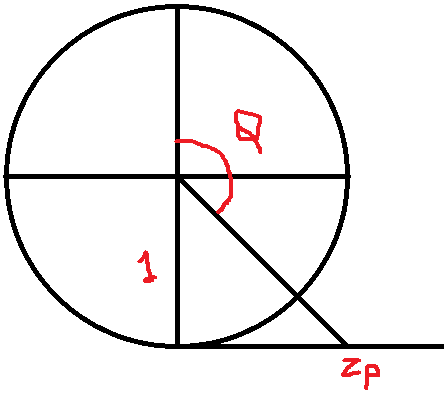
\includegraphics[scale=0.7]{6_14}
    \label{6_14}
\end{figure}

\begin{align*}
    z_p &= -2\tan(\phi/2)/(1-\tan^2(\phi/2))e^{i\theta} \\
    &= 2\cot(\phi/2)e^{i\theta}/(1-\cot^2(\phi/2))\\
    &= 2z_s/(1-|z_s|^2)    
\end{align*}

\tf{(ii)} Circles on hemisphere about the vertical axis originating from $S$. arcs of circles originating from $S$. Plane containing a circular cross section and plane containing an arc of above type, are orthogonal.\\~\\

\begin{figure}[h!]
    \centering
    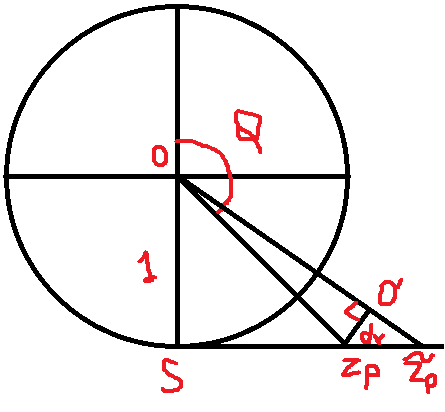
\includegraphics[scale=0.7]{6_14_2}
    \label{6_14_2}
\end{figure}

\tf{(iii)} As in the figure, we have, $OS\td{z_p} \sim z_pO'\td{z_p}$ so that $O'z_p = z_p\td{z_p}OS/O\td{z_p} = Rdr/\sqrt{R^2+r^2}$. Now using $d\hat{s_r}/R = O'z_p/\sqrt{R^2+r^2}$ we get $d\hat{s_r} = R^2dr/(R^2+r^2)$.\\~\\

\begin{figure}[h!]
    \centering
    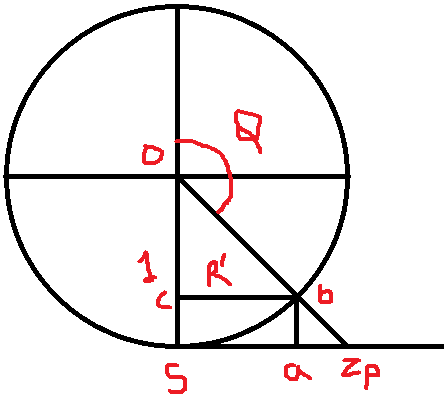
\includegraphics[scale=0.7]{6_14_3}
    \label{6_14_3}
\end{figure}

\tf{(iv)} $d\hat{s_{\theta}} = R'd\theta$. Using above figure, we have $OSz_p \sim Ocb$ so that $cb = Rr/\sqrt{R^2+r^2}$. SO, $d\hat{s_{\theta}} = rd\theta/\sqrt{1+(r/R)^2}$.\\~\\

\tf{(v)} $d\hat{s}^2 = dr^2/(1+(r/R)^2)^2 + r^2d\theta^2/(1+(r/R)^2)$\\~\\

\tf{(vi)} $d\hat{s}^2 = dr^2/(1-r^2) + r^2d\theta^2/(1-r^2)$.

\vspace{0.2in}
%%%%%%%%%%%%%%%%%%%%%%%%%%%%%%%%%

${\textbf{Ex. 6.\theexno}}$
\addtocounter{exno}{1}

Practical.

\vspace{0.2in}
%%%%%%%%%%%%%%%%%%%%%%%%%%%%%%%%%

${\textbf{Ex. 6.\theexno}}$
\addtocounter{exno}{1}

\tf{(i)} The $h$-line in upper half-plane that extends up to infinity is a vertical lines. This corresponds to $x=$const. which corresponds to tractrix generator.\\~\\

\begin{figure}[h!]
    \centering
    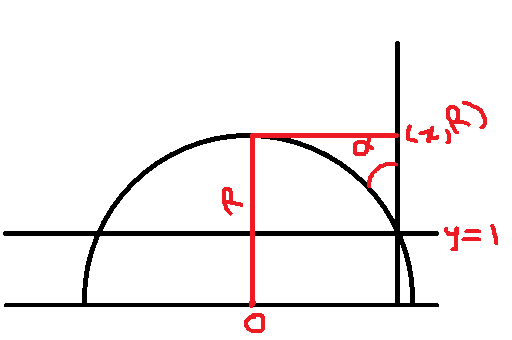
\includegraphics[scale=0.7]{6_16}
    \label{6_16}
\end{figure}

\tf{(ii)} WLOG let the $h$-line (a semicircle) be centred at $0$ and be of radius $R$. Clearly, $\tan\alpha = -dx/dy|_{y=1} = y/\sqrt{R^2-y^2}|_{y=1} = 1/(R^2-1)$. So, $R = 1/\sin\alpha$ and so $|\ln(R/1)| = |\ln(\sin\alpha)|$.

\vspace{0.2in}
%%%%%%%%%%%%%%%%%%%%%%%%%%%%%%%%%

${\textbf{Ex. 6.\theexno}}$
\addtocounter{exno}{1}

$\partial_{x}\ln(\Lambda) = 1/\Lambda \partial_x\Lambda$ and $\partial_{x}^{2}\ln(\Lambda) = -1/(\Lambda)^2(\partial_{x}\Lambda)^2 + 1/\Lambda(\partial_{x}^{2}\Lambda)$.

\tf{(i)} $\Lambda(x,y)=2/(1+x^2+y^2)$ then $\partial_{x}\Lambda =-x \Lambda^2$ and $\partial_x^2 \Lambda = -\Lambda^2 +2x^2\Lambda^3 = (3x^2-y^2-1)\Lambda^3/2$. So, $\partial_{x}^{2}\ln(\Lambda) = -x^2\Lambda^2 + (3x^2-y^2-1)\Lambda^2/2 = (x^2-y^2-1)\Lambda^2/2$. By symmetry, $\partial_{y}^{2}\ln(\Lambda) = (y^2-x^2-1)\Lambda^2/2$. So, $\Delta(\ln(\Lambda)) = -\Lambda^2$. So, $k = 1$ which equals $1/R^2=1/1^2 = 1$.\\~\\

\tf{(ii)} $\Lambda(x,y) = 1/y$ then $\partial_{y}\Lambda = -\Lambda^2$ and $\partial_{y}^{2}\Lambda = 2\Lambda^3$. So, $\partial_{y}^2\ln(\Lambda) = -\Lambda^2 +2\Lambda^2 = \Lambda^2$. So, $\Delta(\ln(\Lambda)) = \Lambda^2 + 0 = \Lambda^2$. So, $k=-1$ as was meant to be.\\~\\

\tf{(iii)} $\Lambda(x,y)=2/(1-x^2-y^2)$ then $\partial_{x}\Lambda =x \Lambda^2$ and $\partial_x^2 \Lambda = \Lambda^2 +2x^2\Lambda^3 = (1+3x^2-y^2)\Lambda^3/2$. So, $\partial_{x}^{2}\ln(\Lambda) = -x^2\Lambda^2 + (1+3x^2-y^2)\Lambda^2/2 = (1+x^2-y^2)\Lambda^2/2$. By symmetry, $\partial_{y}^{2}\ln(\Lambda) = (1+y^2-x^2)\Lambda^2/2$. So, $\Delta(\ln(\Lambda)) = \Lambda^2$. So, $k = -1$ as was meant to be.

\vspace{0.2in}
%%%%%%%%%%%%%%%%%%%%%%%%%%%%%%%%%

${\textbf{Ex. 6.\theexno}}$
\addtocounter{exno}{1}

\begin{figure}[h!]
    \centering
    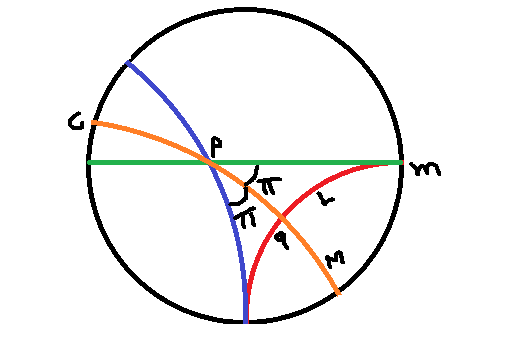
\includegraphics[scale=0.7]{6_18}
    \label{6_18}
\end{figure}

[TODO 6.18]

\vspace{0.2in}
%%%%%%%%%%%%%%%%%%%%%%%%%%%%%%%%%

${\textbf{Ex. 6.\theexno}}$
\addtocounter{exno}{1}

$w = (iz+1)/(z+i)$ so that $|dw| = |D'(z)||dz|$. $D'(z) = -2/(z+i)^2$ so that $|dw| = |D'(z)||dz| = 2|dz|/|z+i|^2$. So, $2|dw|/(1-|w|^2) = \frac{4|dz|/|z+i|^2}{1-(|iz+1|^2/|z+i|^2)} = \frac{4|dz|}{2i(\bar{z}-z)} = |dz|/\mf{Im}z = d\hat{s}$.

\vspace{0.2in}
%%%%%%%%%%%%%%%%%%%%%%%%%%%%%%%%%

${\textbf{Ex. 6.\theexno}}$
\addtocounter{exno}{1}

$M_a^{\phi}(z) = e^{i\phi}(z-a)/(\bar{a}z-1)$. So $|dw| = (||a|^2-1|)/|\bar{a}z-1|^2|dz| = (1-|a|^2)/|\bar{a}z-1|^2|dz|$. $2|dw|/(1-|w|^2) = 2(1-|a|^2)|dz|/((1-|z|^2)(1-|a|^2)) = 2|dz|/(1-|z|^2)$.

\vspace{0.2in}
%%%%%%%%%%%%%%%%%%%%%%%%%%%%%%%%%

${\textbf{Ex. 6.\theexno}}$
\addtocounter{exno}{1}

\tf{(i)} $ai+b = i(ci+d) = -c+id$. So, $a=d$ and $c=-b$. Also, $(a(-bi+a)+b(ai+b))/(-b+ia)^2 = e^{i\phi}$, so that, $(b^2-a^2-2iab)/(a^2+b^2) = e^{-i\phi}$. So, $\cos\phi = (b^2-a^2)/(a^2+b^2)$ and $2ab/(a^2+b^2) = \sin\phi$. Let $a/\sqrt{a^2+b^2} = \cos\theta$. So, $\sin 2\theta = \sin\phi$. So, $\theta = \phi/2$.\\~\\

\tf{(ii)} Using \tf{16 (ii)} we have radius of $B$ is $1/s$ and centre is $\sqrt{1/s^2-1} = -c/s$ (see figure in \tf{(16(ii))}). So, $\Re_{B}(z) = (1/s^2-c^2/s^2 - \bar{z}c/s)/(\bar{z}+c/s) = (s-\bar{z}c)/(c+s\bar{z})$. $\Re_{A}(z) = \lim_{R\rto\infty}(R^2-R^2+\bar{z}R)/(\bar{z}-R) = -\bar{z}$. So, $\Re_{B}\circ\Re_{A}(z) = (zc+s)/(-sz+c)$.\\~\\

\tf{(iii)} $w = (iz+1)/(z+i)$, $wz+iw = iz+1$ so, $z = (1-iw)/(w-i)$. So, $D^{-1}(z) = (1-iw)/(w-i)$. So, $\mc{R}_{i}^{\phi}\circ D^{-1}(z) = (c(1-iz)/(z-i)+s)/(-s(1-iz)/(z-i)+c) = (c-icz + sz-is)/(-s+isz + cz-ic)$. FInally, $D\circ \mc{R}_{i}^{\phi}\circ D^{-1}(z) = (i(c-icz+sz-is)+(-s+isz+cz-ic))/((c-icz+sz-is)+i(-s+isz+cz-ic)) = (ic+cz+isz+s-s+isz+cz-ic)/(c-icz+sz-is -is -sz +icz +c) = z(c+is)/(c-is) = ze^{i\phi/2}/e^{-i\phi/2}$.\\~\\

$[i,1;1,i][\mc{R}_{i}^{\phi}] = [e^{i\phi/2},0;0,e^{-i\phi/2}][i,1;1,i]$. So, $[\mc{R}_{i}^{\phi}] = 1/i\sqrt{2}[i,-1;-1,i][e^{i\phi/2},0;0,e^{-i\phi/2}][i,1;1,i] = 1/i\sqrt{2}[ie^{i\phi/2},-e^{-i\phi/2};-e^{i\phi/2},ie^{-i\phi/2}][i,1;1,i] = 1/i\sqrt{2}[-2c,-2s;2s,-2c]$. So, $\mc{R}_{i}^{\phi} = (cz+s)/(-sz+c)$

\vspace{0.2in}
%%%%%%%%%%%%%%%%%%%%%%%%%%%%%%%%%

${\textbf{Ex. 6.\theexno}}$
\addtocounter{exno}{1}

\tf{(i)} Inverting in a circle centred at $A$ of radius $|a-A|$, we get, $\td{b} = (|a-A|^2-A^2+\bar{b}A)/(\bar{b}-A)$ Also, $\td{B} = (|a-A|^2-A^2+AB)/(B-A)$ so that,

\begin{align*}
    \mc{H}\{a,b\}&= \ln\frac{|a-\td{B}|}{|\td{b}-\td{B}|}\\
    &= \ln\frac{|a-\frac{|a-A|^2-A^2+BA}{B-A}|}{|\frac{|a-A|^2-A^2+\bar{b}A}{\bar{b}-A}-\frac{|a-A|^2-A^2+BA}{B-A}|}\\
    &= \ln \frac{|\bar{b}-A||aB-aA-|a-A|^2+A^2-BA|}{|a-A|^2|B-\bar{b}|}\\
    &= \ln\frac{|\bar{b}-A||(a-A)(B-A-(\bar{a}-A))|}{|a-A|^2|B-\bar{b}|}\\
    &= \ln\frac{|b-A||a-B|}{|a-A||b-B|}\\
    &= \ln|[a,B,b,A]|
\end{align*}

\tf{(ii)} Computing $D^{-1}$ for each point, and putting in the formula, we get,

\begin{align*}
    \mc{H}\{a,b\} &= \ln[D^{-1}(a),D^{-1}(B),D^{-1}(b),D^{-1}(A)]\\
    &= \ln[D^{-1}(a),D^{-1}(B),D^{-1}(b),D^{-1}(A)]\\
    &= \ln|\frac{(\frac{1-ia}{a-i} - \frac{1-iB}{B-i})(\frac{1-ib}{b-i} - \frac{1-iA}{A-i})}{(\frac{1-ia}{a-i} - \frac{1-iA}{A-i})(\frac{1-ib}{b-i} - \frac{1-iB}{B-i})}|\\
    &= \ln |\frac{\frac{2(B-a)}{(a-i)(B-i)}\frac{2(A-b)}{(b-i)(A-i)}}{\frac{2(A-a)}{(a-i)(A-i)}\frac{2(B-b)}{(b-i)(B-i)}}|\\
    &= \ln |\frac{\frac{2(B-a)}{(a-i)(B-i)}\frac{2(A-b)}{(b-i)(A-i)}}{\frac{2(A-a)}{(a-i)(A-i)}\frac{2(B-b)}{(b-i)(B-i)}}|\\
    &= \ln |\frac{(a-B)(b-A)}{(a-A)(b-B)}|
\end{align*}

\vspace{0.2in}
%%%%%%%%%%%%%%%%%%%%%%%%%%%%%%%%%

${\textbf{Ex. 6.\theexno}}$
\addtocounter{exno}{1}

\tf{(i)} $(Aa+B)/(-\bar{B}a+\bar{A}) = 0$ so that $Aa+B = 0$ and $B = -Aa$. So, $M(z) = (Az-Aa)/(\bar{A}\bar{a}z+\bar{A}) = e^{i\psi}(z-a)/(\bar{a}z+1) = \cot(\phi/2)e^{i\theta}$. So, $\cot(\phi/2) = |z-a|/|\bar{a}z+1|$. So, $\pi/2-\phi/2 = \tan^{-1}|(z-a)/(\bar{a}z+1)|$. Required distance is $(\pi-\phi)\cdot 1 = \pi-\phi$.\\~\\

\tf{(ii)} $\mc{H}\{a,z\} = \ln((1+|z-a|/|\bar{a}z-1|)/(1-|z-a|/|\bar{a}z-1|)) = 2\tanh^{-1}(|(z-a)/(\bar{a}z-1)|)$.

\vspace{0.2in}
%%%%%%%%%%%%%%%%%%%%%%%%%%%%%%%%%

${\textbf{Ex. 6.\theexno}}$
\addtocounter{exno}{1}

\tf{(i)} Reflection in the vertical line through $0$.\\~\\

\tf{(ii)} [TODO 6.24]

\vspace{0.2in}
%%%%%%%%%%%%%%%%%%%%%%%%%%%%%%%%%

${\textbf{Ex. 6.\theexno}}$
\addtocounter{exno}{1}

[TODO 6.25]

\vspace{0.2in}
%%%%%%%%%%%%%%%%%%%%%%%%%%%%%%%%%

${\textbf{Ex. 6.\theexno}}$
\addtocounter{exno}{1}

[TODO 6.26]

\vspace{0.2in}
%%%%%%%%%%%%%%%%%%%%%%%%%%%%%%%%%

${\textbf{Ex. 6.\theexno}}$
\addtocounter{exno}{1}

[TODO 6.27]

\vspace{0.2in}
%%%%%%%%%%%%%%%%%%%%%%%%%%%%%%%%%

\clearpage
\setcounter{exno}{1}

\begin{center}
    \textbf{\large{7. Winding Numbers and Topology}}
\end{center}


${\textbf{Ex. 7.\theexno}}$
\addtocounter{exno}{1}

For simple loops, for interior points $N$ must be odd and for exterior points $N$ must be even.

\vspace{0.2in}
%%%%%%%%%%%%%%%%%%%%%%%%%%%%%%%%%

${\textbf{Ex. 7.\theexno}}$
\addtocounter{exno}{1}

\tf{(i)} $e^{i\Phi(\theta)} = e^{iA}$ implies that $\Phi(\theta) = A + 2n\pi$ where $n \in \Z$.\\~\\

\tf{(ii)} 

\vspace{0.2in}
%%%%%%%%%%%%%%%%%%%%%%%%%%%%%%%%%

${\textbf{Ex. 7.\theexno}}$
\addtocounter{exno}{1}

\vspace{0.2in}
%%%%%%%%%%%%%%%%%%%%%%%%%%%%%%%%%

${\textbf{Ex. 7.\theexno}}$
\addtocounter{exno}{1}

\tf{(i)} Checkout video.\\~\\

\tf{(ii)} Suppose $p$ is not a critical point and $\Gamma$ be a circle passing through $p$, and the shape at $f(p)$ of $f(\Gamma)$ is $\prec$. Note that the two infinitesimal small vectors emanating from $p$ came closer (angle between them decreased) as they went through the mapping. This contradicts the fact that the image vectors must be amplitwisted version of input vectors (after translation to $f(p)$). So, $p$ must be critical. Locally curshing effect at critical point? [TODO]\\~\\

\tf{(iii)} $f'(z)$ is a quaratic in $z$ having two roots. So, $f'(z)$ is typically zero at two distinct points and that's when a $\prec$ is produced.\\~\\

\tf{(iv)} Ellipse being a conic section has $5$ degrees of freedom. By just specifying three tangent lines and two points of intersection, we have used all degrees of freedom, and therefore the ellipse must be unique.\\~\\

\tf{(v)} Approach: Take the two critical points of

\vspace{0.2in}
%%%%%%%%%%%%%%%%%%%%%%%%%%%%%%%%%

${\textbf{Ex. 7.\theexno}}$
\addtocounter{exno}{1}

$f(z) = e^{i\pi/4}z$. Then, local linear transformation produced by the mapping at $a$ will have $\xi_a=1$, $\eta_a=1$ and $\phi_a = \pi/4$. However, $f(x,y) = (x+iy)(1+i)/\sqrt{2} = [(x-y)+i(x+y)]/\sqrt{2}$,
\begin{align*}
    J(a) &= \frac{1}{\sqrt{2}}\begin{bmatrix}1&-1\\1&1\end{bmatrix}\\
    \lambda_1, \lambda_2 &= (1\pm i)/sqrt{2}\\
    \det J(a) &= 1\\
    \lambda_1\lambda_2 &= 1\\
    \xi\eta &= 1
\end{align*}

\vspace{0.2in}
%%%%%%%%%%%%%%%%%%%%%%%%%%%%%%%%%

${\textbf{Ex. 7.\theexno}}$
\addtocounter{exno}{1}

Complex eigenvalues must occur in conjugate pairs and therefore the product of two nonzero conjugate pairs will be positive. So, the sign of $\det J(a)$ depends on the number of negative real eigenvalues, $n$ and $\nu(a)$ is therefore, $(-1)^n$.

\vspace{0.2in}
%%%%%%%%%%%%%%%%%%%%%%%%%%%%%%%%%

${\textbf{Ex. 7.\theexno}}$
\addtocounter{exno}{1}

\tf{(i)} $z\bar{z}-i\bar{z}=\bar{z}(z-i) = 0 \iff z = 0,i$.\\~\\

\tf{(ii)} $h(x,y) = x^2+y^2 -ix -y$. $J = \begin{bmatrix}2x&2y-1\\-1&0\end{bmatrix}$ and $\det J = 2y-1$.\\~\\

\tf{(iii)} $\det J(0) = -1$ and $\det J(i) = 1$. So multiplicity of $0$ is $-1$ and that of $i$ is $1$.\\~\\

\tf{(iv)} For $|z|=2$, $h(z)=4-i2e^{-i\theta}$. Take the initial circle, flip it about the real axis, rotate it by $-\pi/2$ and then translate it towards positive real axis by $4$ units. The result is $|z-4|=2$. Since $0$ is outside the resulting the circle, $\nu[h(C),0]=0$ which can be confirmed by adding the multiplicities of its preimages inside $C$ which are $0$ (multiplicity $-1$) and $i$ (multiplicity $1$).\\~\\

\tf{(v)} Consider a small circle containing $0$ and not containing $i$. Then as $z$ traverses this circle counterclockwise, $\bar{z}$ will traverse the same circle in opposite direction and $z-i$ will ultimately have a net rotation fo $0$ about $0$. So, windining number of $h(z)$ about $0$ is $-1$. Similarly winding number of $h(z)$ about $i$ is $1$. Finally, as $z$ traverses the circle $C_2$, $\bar{z}$ will have net rotation of $-2\pi$ and $z-i$ will have net rotation of $2\pi$, so, $h(z)$ has net rotation of $0$ about $0$.\\~\\

\tf{(vi)} Note that $\det J(i/2)=0$ and $f(i/2) = -1/2$. Consider a small circle about $i/2$. $\bar{z}$ will lead to a rotation of $-2\pi$ about $-1/2$ and $z-i$ will lead to a rotation of $2\pi$ about $-1/2$ leading to a net rotation of $0$. So, the image of the circle will lead to a loop s.t. $-1/2$ is outside the loop.

\vspace{0.2in}
%%%%%%%%%%%%%%%%%%%%%%%%%%%%%%%%%

${\textbf{Ex. 7.\theexno}}$
\addtocounter{exno}{1}

$F(s) = \prod_{i=1}^{n}(s-s_j)$. $\Rto$ Suppose all $s_j$ are s.t. $\mf{Re}(s_j)<0$. Consider the left sided semicircle containing the segment from $-iR$ to $iR$ as diameter. If $s_j$ lies inside this semicircle loop, then the vector $s-s_j$ makes a rotation of $\pi$ as $s$ traverses the semicircle arc. By argument principle, the total rotation made by $s-s_j$ as $s$ traverses the loop must be $2\pi$, so, the rotation made by $s-s_j$ as $s$ traverses from $-iR$ to $iR$ will also be $\pi$ (this can also be seen directly). Now, as $R\rto\infty$ all $s_j$ will be contained in the semicircle loop, and since for the product of complex numbers the arguments add up, the net rotation made by $F(s)$ as $s$ traverses from $-iR$ to $iR$ is $n\pi$.\\~\\

$\Lto$ Suppose $\mc{R}=n\pi$ and $s_i$ lies on the left half plane. The contribution to the net rotation of $F(s)$ by $s_j$ will be $-\pi$ (by above argument). Since no $s-s_j$ cannot make a rotation greater than $\pi$ for any $s_j$ as $s$ traverses from bottom to top of imaginary axis, the net rotation must be $\leq (n-1)\pi$. Contradiction.

\vspace{0.2in}
%%%%%%%%%%%%%%%%%%%%%%%%%%%%%%%%%

${\textbf{Ex. 7.\theexno}}$
\addtocounter{exno}{1}

\tf{(i)} $F(s)=s^3-1=0$. As $s$ traverses from bottom to top of imaginary axis, $s^3-1$ traverses from the top to the bottom of a line parallel to imaginary axis passing through $-1+0i$. Therefore $\mc{R}=\pi \neq 3\pi$ and the Nyquist Stability Criterion is not satisfied.\\~\\

\tf{(ii)} Solutions are $1,e^{i2\pi/3},e^{i4\pi/3}$. Two of them lie in the left-half plane, one lies in the right-half plane. So, general solution does not decay with $t$. Also, net rotation of $F(s)$ is $2\pi-\pi=\pi$.

\vspace{0.2in}
%%%%%%%%%%%%%%%%%%%%%%%%%%%%%%%%%

${\textbf{Ex. 7.\theexno}}$
\addtocounter{exno}{1}

$z^ne^a - e^z = 0$. Let $f(z)=z^n$ and $g(z) = -e^{z-a}$. On the unit circle,

\begin{align*}
    |g(z)| &= |e^{z-a}|\\
    &= |e^{\cos\theta-a}|\\
    &\leq |e^{1-a}|\\
    &<1 \qquad (\because a > 1)\\
    &=|f(z)| 
\end{align*}

\vspace{0.2in}
%%%%%%%%%%%%%%%%%%%%%%%%%%%%%%%%%

${\textbf{Ex. 7.\theexno}}$
\addtocounter{exno}{1}

\tf{(i)} Let $f(z) = 2z^5$ and $g(z) = 8z-1$. Then, on the disc $|z|=2$, we have,

\begin{align*}
    |g(z)| &= |8z-1|\\
    &= |16\cos\theta-1 + 16i\sin\theta|\\
    &= \sqrt{(16\cos\theta-1)^2 + (16\sin\theta)^2}\\
    &= \sqrt{16^2 + 1 - 32\cos\theta}\\
    &\leq \sqrt{16^2+1+32}
    &= 17\\
    &< 64\\
    &= |f(z)|
\end{align*}

\tf{(ii)} On the unit disc $|z|=1$,

\begin{align*}
    |g(z)| &= |8z-1|\\
    &= \sqrt{8^2+1-16\cos\theta}\\
    &\geq 7\\
    &> 2\\
    &= |f(z)|
\end{align*}

\vspace{0.2in}
%%%%%%%%%%%%%%%%%%%%%%%%%%%%%%%%%

${\textbf{Ex. 7.\theexno}}$
\addtocounter{exno}{1}

\tf{(i)} Number of preimages (counted with their multiplicities) of $0$ in $\Gamma$ of $p(z)$ is $\nu[p(\Gamma),0]$ and that of $q(z)$ is $\nu[q(\Gamma),0]$. So total number of preimages (counted with their multiplicities) of $0$ in $\Gamma$ of $p(z)q(z)$ is the sum $\nu[p(\Gamma),0] + \nu[p(\Gamma),0]$. Suppose their is an overlap of the preimage i.e. $p$ be the preimage of $0$ in $p(z)$ and $q(z)$ then its multiplicity for $p(z)q(z)$ will be sum of individual multiplicities (this can be observed by computing net rotation of $p(z)q(z)$ about $0$ due to $p$ and the fact that: product of complex numbers leads to addition of arguments).\\~\\

\tf{(ii)} Note that $|g(z)/f(z)| < 1$. So, for a typical loop $\Gamma$, the image loop through $g(z)/f(z)$ will lie strictly inside the unit circle and therefore $1+g(z)/f(z)$ will lie strictly in the disc $|z-1|<1$. Note that $0$ will be outside of the image loop and therefore $\nu[H(\Gamma),0] = 0$.\\~\\

\tf{(iii)} If $f+g\neq$ then $1+g/f \neq 0$, so again $0$ will be outside of image loop even through image loop lies inside $|z-1|\leq 1$.

\vspace{0.2in}
%%%%%%%%%%%%%%%%%%%%%%%%%%%%%%%%%

${\textbf{Ex. 7.\theexno}}$
\addtocounter{exno}{1}

\tf{(i)} Due to analyticity we have $f(z+\Delta)-f(z) = f'(z)\Delta$. Given that the image loop is origin centered circle, we have $f(z+\Delta)=f(z)e^{i\phi}$. So, $f'\Delta = f(e^{i\phi}-1) = f(\cos\phi - 1 + i\sin\phi) = fi\phi$ because $\phi$ is very close to $0$.\\~\\

\tf{(ii)} Collecting all $\Delta$ and plotting them from origin, one would obtain a simple loop by joining the other end points of all $\Delta$s therefore $\nu[\Delta,0] = 1$. On the other hand, all $i\phi$ vectors will lie on the imaginary axis and therefore as $z$ traverses $\Gamma$, one never completes a rotation of $2\pi$ about $0$ (infact the angle would be $0$).\\~\\

\tf{(iii)}

\begin{align*}
    \nu[f(\Gamma),0] + \nu[i\phi,0] = \nu[f'(\Gamma),0] + \nu[\Delta,0]
\end{align*}

\tf{(iv)} Since $f$ is analytic, $f$ must have one more preimage of $0$ inside $\Gamma$ than the number of preimages of $0$ in $f'$ inside $\Gamma$.\\~\\

\tf{(v)} The modular surface of $f$ will be constant above $\Gamma$. Since for an analytic function, the interior of $\Gamma$ will be in one-to-one correspondence with the interior of the circle, there will be one point inside $\Gamma$ mapping to $0$. [TODO:There should be exactly one root].

\vspace{0.2in}
%%%%%%%%%%%%%%%%%%%%%%%%%%%%%%%%%

${\textbf{Ex. 7.\theexno}}$
\addtocounter{exno}{1}

\tf{(i)} $\phi$ maps the interior of disc of radius $1/2$ to origin and maps the leftover interior of disc of radius $1$ to a circle of unit radius.\\~\\

\tf{(ii)} Image of $\Gamma$ is a circle of radius $1/2$ centered at origin. So, the winding number of $f(\Gamma)$ about $0$ should be $1$. But, there are infinitely many preimages $0$ inside $\Gamma$ and associating a multiplicity for these preimages is not possible by the definition of topological multiplicity argument (we can not form a small circle containing a single preimage).

\vspace{0.2in}
%%%%%%%%%%%%%%%%%%%%%%%%%%%%%%%%%

${\textbf{Ex. 7.\theexno}}$
\addtocounter{exno}{1}

\tf{(i)} Since, on unit circle, $|g(z)| \leq 1 = |-z| = |f(z)|$ and $f+g\neq 0$ on the unit circle, we have by Ex.\tf{12.(iii)} that $\nu[m(C),0] = \nu[f(z),0] = 1$.\\~\\

\tf{(ii)} [TODO].

\vspace{0.2in}
%%%%%%%%%%%%%%%%%%%%%%%%%%%%%%%%%

${\textbf{Ex. 7.\theexno}}$
\addtocounter{exno}{1}

Because $f(p)$ points in the opposite direction of $f(-p)$, net rotation of $f(z)$ as $z$ traverses from $p$ to $-p$ will be of form $2n\pi + \pi$ where $n\in\Z$. The remaining semicircle traversal is traversal of $-z$ as $z$ traverses from $p$ to $-p$. Since $f(-p)=-f(p)$, the image of this traversal will be reflection about $0$ of the image of the first semicircle. Therefore, as $f(z)$ makes a rotation of $\theta$ about origin $f(-z)=-f(z)$ will also make a rotation of $\theta$ about origin in same sense. Therefore, net rotation due to remaining semicircle is also $2n\pi+\pi$. Total rotation is $2\pi(2n+1)$, so winding number is $2n+1$.

\vspace{0.2in}
%%%%%%%%%%%%%%%%%%%%%%%%%%%%%%%%%

${\textbf{Ex. 7.\theexno}}$
\addtocounter{exno}{1}

$F(p) = H(p)-H(p^*)$ and $F(-p) = F(p^*) = H(p^*) - H(p)$. So, $F(p)$ and $F(-p)$ point in opposite directions. Taking the circle $C$ as in question and from previous exercise we have $\nu[F(C),0]=\text{odd}$. Therefore, $\nu[H(C),0]\neq 0$.

\vspace{0.2in}
%%%%%%%%%%%%%%%%%%%%%%%%%%%%%%%%%

${\textbf{Ex. 7.\theexno}}$
\addtocounter{exno}{1}



\vspace{0.2in}
%%%%%%%%%%%%%%%%%%%%%%%%%%%%%%%%%

${\textbf{Ex. 7.\theexno}}$
\addtocounter{exno}{1}

\vspace{0.2in}
%%%%%%%%%%%%%%%%%%%%%%%%%%%%%%%%%

${\textbf{Ex. 7.\theexno}}$
\addtocounter{exno}{1}

\vspace{0.2in}
%%%%%%%%%%%%%%%%%%%%%%%%%%%%%%%%%

${\textbf{Ex. 7.\theexno}}$
\addtocounter{exno}{1}

\vspace{0.2in}
%%%%%%%%%%%%%%%%%%%%%%%%%%%%%%%%%

${\textbf{Ex. 7.\theexno}}$
\addtocounter{exno}{1}

\vspace{0.2in}
%%%%%%%%%%%%%%%%%%%%%%%%%%%%%%%%%


\clearpage
\setcounter{exno}{1}

\begin{center}
    \textbf{\large{8. Complex Integration: Cauchy's Theorem}}
\end{center}

${\textbf{Ex. 8.\theexno}}$\addtocounter{exno}{1}\\~\\
\tf{(i)}

\begin{align*}
    v(x) &= \frac{dz(x)}{dx}\\
    &= 1 + if'(x)\\
    &= 1 + i\tan\theta
\end{align*}

\begin{align*}
    a(x) &= \frac{d^2z(x)}{dx^2}\\
    &= if''(x)
\end{align*}

\tf{(ii)}

\begin{align*}
    \Im(a\bar{v}) &= f''(x)\\
    |v|^{3} &= (1+\tan^2\theta)^{3/2} = \sec^3\theta\\
    \kappa = f''(x)/\sec^3\theta
\end{align*}

\tf{(iii)}

\begin{align*}
    \text{area}(ABCD) = \frac{1}{8}\kappa\sec^3\theta \Delta^3 = \frac{1}{8}f''(x)\Delta^3
\end{align*}

\vspace{0.2in}
%%%%%%%%%%%%%%%%%%%%%%%%%%%%%%%%%

${\textbf{Ex. 8.\theexno}}$\addtocounter{exno}{1}

\vspace{0.2in}
%%%%%%%%%%%%%%%%%%%%%%%%%%%%%%%%%

${\textbf{Ex. 8.\theexno}}$\addtocounter{exno}{1}

\vspace{0.2in}
%%%%%%%%%%%%%%%%%%%%%%%%%%%%%%%%%

${\textbf{Ex. 8.\theexno}}$\addtocounter{exno}{1}
\tf{(i)} Singular point $0$ is inside $L$. $I=2\pi i\nu[L,0] = 2\pi i$. Parametric form of $L$ is $z(t) = e^{it}$ where $t \in [0,2\pi)$ and $dz(t) = ie^{it}dt$.

\begin{align*}
    I &= \int_{0}^{2\pi}(1/e^{it})ie^{it}dt\\
    &= i\int_{0}^{2\pi}dt\\
    &= 2\pi i
\end{align*}
\tf{(ii)} Singular point $0$ is outside $L$. So, $I=2i\pi\nu[L,0] = 0$. Parametric form of $L$ is $z(t) = 2+e^{it}$ where $t \in [0,2\pi)$ and $dz(t) = ie^{it}dt$.

\begin{align*}
    I &= \int_{0}^{2\pi}\frac{1}{2+e^{it}}ie^{it}dt\\
    &= i\int_{0}^{2\pi}\left(1-\frac{2}{2+\cos t + i\sin t}\right)dt\\
    &= 2\pi i -2i \int_{0}^{2\pi}\frac{2+\cos t + i\sin t}{5+4\cos t}dt\\
    &= 2\pi i - 2i(\pi + i0)\\
    &= 0
\end{align*}

\tf{(iii)} Singular point $0$ is inside $L$. $I=2\pi i\nu[L,0] = 2\pi i$. Parametric form of $L$ is $z(t) = 1+2e^{it}$ where $t \in [0,2\pi)$ and $dz(t) = 2ie^{it}dt$.

\begin{align*}
    I &= \int_{0}^{2\pi}\frac{1}{1+2e^{it}}2ie^{it}dt\\
    &= i\int_{0}^{2\pi}\left(1-\frac{1+2\cos t - 2i\sin t}{5 + 4\cos t}\right)\\
    &= 2\pi i - i(0 + i0)\\
    &= 2\pi i
\end{align*}

\vspace{0.2in}
%%%%%%%%%%%%%%%%%%%%%%%%%%%%%%%%%

${\textbf{Ex. 8.\theexno}}$\addtocounter{exno}{1}
Parametric form of $L$ consists of $L_1 \equiv z(t) = 1+it, t\in [-1,1]$, $L_2 \equiv z(t) = -t+i, t \in [-1,1]$, $L_3 \equiv z(t) = -1-it, t\in [-1,1]$ and $L_3 \equiv z(t) = t - i, t\in [-1,1]$.

\begin{align*}
    I &= \int_{-1}^{1}(i/(1+it) - 1/(-t+i) -i/(-1-it) + 1/(t-i))dt\\
    &= 4\int_{-1}^{1}(i+t)/(1+t^2)dt\\
    &= 2\log(1+t^2)|_{-1}^{1} + 4i\tan^{-1}(t)|_{-1}^{1}\\
    &= 4i\pi/2\\
    &= 2\pi i
\end{align*}

\vspace{0.2in}
%%%%%%%%%%%%%%%%%%%%%%%%%%%%%%%%%

${\textbf{Ex. 8.\theexno}}$\addtocounter{exno}{1}
Parametric form of $L$ is $z(t) = Ae^{it}$ where $t \in [0,2\pi)$. So, $dz(t) = Aie^{it}dt$.

\begin{align*}
    I &= \int_{0}^{2\pi}A^{m}e^{imt}Aie^{it}dt\\
    &= i\int_{0}^{2\pi}A^{m+1}e^{i(m+1)t}dt\\
    &= iA^{m+1}\int_{0}^{2\pi}(\cos(m+1)t + i \sin(m+1)t) dt\\
    &= \left\{\begin{matrix}0&m\neq -1\\2\pi i & m = -1\end{matrix}\right.
\end{align*}

\vspace{0.2in}
%%%%%%%%%%%%%%%%%%%%%%%%%%%%%%%%%

${\textbf{Ex. 8.\theexno}}$\addtocounter{exno}{1}
\tf{(i)} When $B$ has rolled by angle $u$, the point on the rim of $B$ touching $A$ would have rotated by an angle $t$ given by $tA = uB$. The centre of $B$ is at $(A+B)e^{iu}$ and the point of the rim being traced will be at $(A+B)e^{iu} + Be^{it}$. When $A=nB$, the parametric form of the point being traced is $z(t) = B((n+1)e^{it}-e^{i(n+1)t})$.\\~\\

\tf{(ii)} $dz(t) = i(n+1)B(e^{it}-e^{i(n+1)t})dt$.

\begin{align*}
I &= \int_{0}^{2\pi} B((n+1)e^{-it}-e^{-i(n+1)t})i(n+1)B(e^{it}-e^{i(n+1)t})dt\\
&= i(n+1)B^2\int_{0}^{2\pi}((n+1) + 1 - (n+1)e^{int} = e^{-int})dt\\
&= 2\pi i(n+1)B^2(n+2)
\end{align*}

Comparing this with $I = 2(\text{area enclosed})$, we get the result.

\vspace{0.2in}
%%%%%%%%%%%%%%%%%%%%%%%%%%%%%%%%%

${\textbf{Ex. 8.\theexno}}$\addtocounter{exno}{1}
\tf{(i)}

\begin{align*}
    I &= \int_{0}^{2\pi}Re^{-it}iRe^{it}dt\\
    &= 2\pi i R^2
\end{align*}

\tf{(ii)} Define $p = (a+b)/2$ and $q = (a-b)/2$ then parametric form of ellipse is $pe^{it} + q^{-it}$.

\begin{align*}
    I &= \int_{0}^{2\pi} (pe^{-it} + qe^{it})i(pe^{it}-qe^{-it})dt\\
    &= i\int_{0}^{2\pi} (p^2 - q^2 + pq(e^{-2it} + e^{2it})) dt\\
    &= 2\pi a b i
\end{align*}

\tf{(iii)}

\begin{align*}
    I &= \int_{0}^{R}tdt + \int_{0}^{\pi/2}Re^{-it}iRe^{it}dt + \int_{R}^{0}(-it)idt\\
    &= R^2/2 + i(\pi/2)R^2 - R^2/2\\
    &= i(\pi/2)R^2
\end{align*}

\tf{(iv)}

\begin{align*}
    I &= \int_{0}^{R}(R-it)idt + \int_{R}^{0}(t - iR)dt + \int_{0}^{1}(tR - (1-t)iR)(R-iR)dt\\
    &= iR^2 + R^2/2 - R^2/2 + iR^2 -iR(R-iR) + R^2\\
    &= iR^2
\end{align*}

\vspace{0.2in}
%%%%%%%%%%%%%%%%%%%%%%%%%%%%%%%%%

${\textbf{Ex. 8.\theexno}}$\addtocounter{exno}{1} Area enclosed by sector subtended by the contour at origin.

\vspace{0.2in}
%%%%%%%%%%%%%%%%%%%%%%%%%%%%%%%%%

${\textbf{Ex. 8.\theexno}}$\addtocounter{exno}{1} Let $L = \sum_{j}\nu_j C_j = \sum_{\text{inside}}\nu_jC_j$ (because $\nu_j = 0$ for outside), where $C_j$ is a simple loop and $\nu_j$ is the common winding number of the points inside $C_j$. Then,

\begin{align*}
    \oint_{L}f(z)dz &= \sum_{\text{inside}}\nu_j\oint_{C_j}f(z)dz\\
    \oint_{L}\bar{z}dz &= \sum_{\text{inside}}\nu_j\oint_{C_j}\bar{z}dz\\
    &= \sum_{\text{inside}}\nu_j(2i A_j)
\end{align*}

\vspace{0.2in}
%%%%%%%%%%%%%%%%%%%%%%%%%%%%%%%%%

${\textbf{Ex. 8.\theexno}}$\addtocounter{exno}{1}

\vspace{0.2in}
%%%%%%%%%%%%%%%%%%%%%%%%%%%%%%%%%

${\textbf{Ex. 8.\theexno}}$\addtocounter{exno}{1}
\tf{(i)} 

\begin{align*}
    \frac{z}{z^2-iz-1-i} &= \frac{1}{5}\frac{2-i}{z+1} + \frac{1}{5}\frac{3+i}{z-1-i}\\
    \oint_{K}\frac{z}{z^2-iz-1-i}dz &= \oint_{K}\frac{1}{5}\frac{2-i}{z+1}dz + \oint_{K}\frac{1}{5}\frac{3+i}{z-1-i}dz\\
    &= (\frac{2-i}{5} 2\pi i (-2)) + (\frac{3+i}{5}2\pi i  (0))\\
    &= -4(2-i)\pi i/5
\end{align*}

\tf{(ii)}

\begin{align*}
    \cos z/z^{11} &= 1/z^{11} - 1/(2!z^{9}) + 1/(4!z^{7}) - 1/(6!z^{5})\\
    &\qquad + 1/(8!z^{3}) - 1/(10!z) + z/(12!) - z^{3}/(14!) + \ldots\\
    \oint_{K}\cos z/z^{11}dz &= -(1/(10!))2\pi (-1) = 2\pi /(10!)
\end{align*}

\vspace{0.2in}
%%%%%%%%%%%%%%%%%%%%%%%%%%%%%%%%%

${\textbf{Ex. 8.\theexno}}$\addtocounter{exno}{1}

\tf{(i)}

\begin{align*}
    z^4+1 &= (z^2+i)(z^2-i)\\
    &= (z-\frac{1-i}{\sqrt{2}})(z-\frac{-1+i}{\sqrt{2}})(z-\frac{1+i}{\sqrt{2}})(z-\frac{-1-i}{\sqrt{2}})\\
    \frac{1}{z^4+1} &= \frac{\ldots}{z-\frac{1-i}{\sqrt{2}}} + \frac{1/(2\sqrt{2}(1+i))}{z-\frac{-1+i}{\sqrt{2}}} + \frac{1/(2\sqrt{2}(-1+i))}{z-\frac{1+i}{\sqrt{2}}} + \frac{\ldots}{z-\frac{-1-i}{\sqrt{2}}}
\end{align*}

Singular points are $(1+i)/\sqrt{2}$, $(1-i)/\sqrt{2}$, $(-1-i)/\sqrt{2}$, $(-1+i)/\sqrt{2}$. If $R < 1$ then no singular point is inside the loop, so integrap vanishes. For $R > 1$, singular points $(1+i)/\sqrt{2}$ and $(-1+i)/\sqrt{2}$ lie inside the loop and will contribute to integral and the value of the integral will be $\frac{1}{2\sqrt{2}}(1/(1+i)+1/(-1+i))2\pi i = \pi/\sqrt{2}$.\\~\\

\tf{(ii)} As $z$ travels around $J$ once, $z^4$ travels around the complete circle of radius $R^4$ with origin as centre twice. Since $z^4+1$ is nothing but a horizontally shifted (by $1$) version of this circle, we have the minimum value of $|z^4+1|$ is $R^4-1$. Therfore, the minimum value of $1/|z^4+1|$ is $1/(R^4-1)$. Also, the length of $J$ is $\pi R$. Using $5$ we have $|\int_{J}f(z)dz| \leq \pi R/(R^4-1)$. As $R \rto \infty$, $I \rto 0$.\\~\\ 

\tf{(iii)} As $R \rto \infty$, all contribution comes from $L$. So, the required value is $\pi/\sqrt{2}$.

\vspace{0.2in}
%%%%%%%%%%%%%%%%%%%%%%%%%%%%%%%%%

${\textbf{Ex. 8.\theexno}}$\addtocounter{exno}{1}
\tf{(i)}

\begin{align*}
    z^2+1 &= (z+i)(z-i)\\
    \frac{1}{z^2+1} &= (i/2)/(z+i) - (i/2)(z-i)
\end{align*}

Singular points are $i$ and $-i$. Singular points inside $L+J$ is $i$. So, $I = -(i/2) \cdot 2\pi i = \pi$. As $R\rto \infty$ integral round $J$ will die with $O(1/R)$.\\~\\

\tf{(ii)}

\begin{align*}
    \frac{1}{(z^2+1)^2} &= (-1/4)/(z+i)^2 - (-1/4)/(z-i)^2 + (1/2)(z+i)(z-i)\\
    &= (-1/4)/(z+i)^2 - (-1/4)/(z-i)^2 + (i/4)/(z+i) - (i/4)(z-i)
\end{align*}

Singular points are $i$ and $-i$. First two integrals will vanish for $L+J$. The only contribution comes from the last term i.e. $-(i/4) \cdot 2\pi i = \pi/2$.

Ordinary way is to put $x=\tan \theta$ and $dx = \sec^2\theta d\theta$ to get, 

\begin{align*}
    I &= \int_{-\pi/2}^{\pi/2}d\theta/\sec^2\theta\\
    &= \int_{-\pi/2}^{\pi/2}\cos^2\theta d\theta\\
    &= \int_{-\pi/2}^{\pi/2}((1+\cos(2\theta))/2)d\theta\\
    &= \pi/2
\end{align*}

\vspace{0.2in}
%%%%%%%%%%%%%%%%%%%%%%%%%%%%%%%%%

${\textbf{Ex. 8.\theexno}}$\addtocounter{exno}{1}

\tf{(i)} $F(z) = e^z$. So, $I=F(a+ib)-F(0) = e^a(\cos b + i \sin b) - 1$.\\~\\

\tf{(ii)} $z(t) = t(a+ib)$ where $t \in [0,1]$. $dz(t) = a+ib$. So,

\begin{align*}
    I &= \int_{0}^{1}e^{t(a+ib)}(a+ib)dt\\
    &= (a+ib)\int_{0}^{1}(e^{at}\cos(bt) + i e^{at}\sin(bt))dt\\
    &= e^{a}(\cos b + i\sin b) - 1
\end{align*}

Equating real and imaginary parts, and solving,

\begin{align*}
    aI_1 -bI_2 &= e^a\cos b - 1\\
    bI_1 + aI_2 = e^a\sin b\\
    I_1 &= (a(e^a\cos b - 1) + b(e^a\sin b))/(a^2+b^2)\\
    I_2 &= (b(1-e^a\cos b) + a(e^a\sin b))/(a^2+b^2)
\end{align*}

\tf{(iii)} Using integration by parts.

\begin{align*}
    I_1 &= \cos bx e^{ax}/a|_{0}^{1} + (b/a) I_2\\
    &= (e^a\cos b)/a - 1/a + (b/a)I_2\\
    I_2 &= \sin bx e^{ax}/a|_{0}^{1} - (b/a)I_1\\
    &= (e^{a}\sin b)/a - (b/a)I_1
\end{align*}

Put second equationg in first to get,

\begin{align*}
    I_1 &= (e^a\cos b)/a - 1/a + (b/a)((e^{a}\sin b)/a - (b/a)I_1)\\
    (1+(b^2/a^2))I_1 &= (a(e^a\cos b - 1) + b(e^a\sin b))/a^2\\
    I_1 &= (a(e^a\cos b - 1) + b(e^a\sin b))/(a^2+b^2)\\
    I_2 &= (e^{a}\sin b)/a - (b/a)I_1\\
    &= (b(1-e^a\cos b) + a(e^a\sin b))/(a^2+b^2)
\end{align*}

\vspace{0.2in}
%%%%%%%%%%%%%%%%%%%%%%%%%%%%%%%%%

${\textbf{Ex. 8.\theexno}}$\addtocounter{exno}{1}

\tf{(i)} [Doubt]

\begin{align*}
    \int_{a}^{b} f(z)g(z)dz &= f(z)G(z)|_{a}^{b} - \int_{a}^{b}f'(z)G(z)dz
\end{align*}

\tf{(ii)}

\begin{align*}
    \int_{L} ze^{iz}dz &= \theta(-ie^{i\theta}) + \theta(-ie^{-i\theta}) + (e^{i\theta} - e^{-i\theta})\\
    &= -2i\theta\cos\theta + 2i\sin\theta\\
    &= 2i(\sin\theta-\theta\cos\theta)
\end{align*}

\begin{align*}
    \int_{-\theta}^{\theta}te^{it}dt = \int_{-\theta}^{\theta}t(\cos t +i\sin t)dt\\
    &= 0 + i(t(-\cos t)|_{-\theta}^{\theta} + \int_{-\theta}^{\theta}\cos tdt)\\
    &= i(-2\theta\cos\theta + 2\sin\theta)
\end{align*}

\vspace{0.2in}
%%%%%%%%%%%%%%%%%%%%%%%%%%%%%%%%%

${\textbf{Ex. 8.\theexno}}$\addtocounter{exno}{1}

\tf{(i)} 

\begin{align*}
    f(z) = (1/z)(\sum_{i=0}^{n}\binom{n}{i}z^{2i-n})
\end{align*}

If $n = 2m$ then, the only term with $-1$ as the power of $z$ has coefficient $\binom{n}{n/2}$ which is the residue at origin. If $n = 2m+1$ then there is no term with $-1$ as the power of $z$. So, no residue at origin in odd case.\\~\\

\tf{(ii)} No residue at origin. So, zero for every loop.\\~\\

\tf{(iii)} $I = 2\pi i \nu[C,0] \text{Res}(f(z),0) = 2\pi i \binom{n}{n/2}$.\\~\\

\tf{(iv)} $z(\theta) = e^{i\theta}$ where $\theta \in [0,2\pi)$ and $dz(\theta) = ie^{i\theta}d\theta$.

\begin{align*}
    \oint_{C}f(z)dz &= \int_{0}^{2\pi}e^{-i\theta}(2\cos\theta)^{2m}ie^{i\theta}d\theta\\
    &= i2^{2m}\int_{0}^{2\pi}\cos^{2m}\theta d\theta\\
\end{align*}

Compare with $\tf{(iii)}$.

\tf{(v)} 

\begin{align*}
    z^kf(z) = (\sum_{i=0}^{n}\binom{n}{i}z^{2i-n + k-1})
\end{align*}

Term has $-1$ as power of $z$ when $2i-n+k-1=-1$ i.e. $2i = n-k$ i.e. $n-k$ must be divisible by $2$. When this is the case, the residue at origin is $\binom{n}{(n-k)/2}$, otherwise residue is zero. The value of integral for a loop round origin will be $2\pi i \binom{n}{n-k}$. Using parameteric form $z(\theta) = e^{i\theta}$ where $\theta \in [0,2\pi)$ and $dz(\theta) = ie^{i\theta}$, we get, (when $n-k$ is divisible by $2$)

\begin{align*}
    \oint z^kf(z)dz &= \int_{0}^{2\pi}e^{i(k-1)\theta}(2\cos\theta)^{n}ie^{i\theta}d\theta\\
    &= 2^n\int_{0}^{2\pi}\cos^n\theta (\cos k\theta + i\sin k\theta)d\theta\\
    &= 2\pi i \binom{n}{n-k}\\
    \int_{0}^{2\pi}\cos^n\theta \cos k\theta d\theta &= 0\\
    &= \int_{0}^{2\pi}\cos^n\theta \sin k\theta d\theta &= \pi/2^{n-1}\binom{n}{n-k}
\end{align*}

\vspace{0.2in}
%%%%%%%%%%%%%%%%%%%%%%%%%%%%%%%%%

${\textbf{Ex. 8.\theexno}}$\addtocounter{exno}{1}

Using Cauchy theorem the value of the integral will be $2\pi i$. Using parameteric evaluation - $z(t) = a\cos t + ib\sin t$ where $t \in [0,2\pi)$ and $dz(t) = (-a\sin t + ib\cos t)dt$, we have,

\begin{align*}
    \oint_{E}(1/z)dz &= \int_{0}^{2\pi}\frac{-a\sin t + ib\cos t}{a\cos t + ib\sin t} dt\\
    &= \int_{0}^{2\pi}\frac{(-a^2+b^2)\cos t\sin t + i(ab\sin^2 t + ab \cos^2 t)}{a\cos t + ib\sin t} dt\\
\end{align*}

Compare the imaginary parts.

\vspace{0.2in}
%%%%%%%%%%%%%%%%%%%%%%%%%%%%%%%%%

${\textbf{Ex. 8.\theexno}}$\addtocounter{exno}{1}



\vspace{0.2in}
%%%%%%%%%%%%%%%%%%%%%%%%%%%%%%%%%

${\textbf{Ex. 8.\theexno}}$\addtocounter{exno}{1}
Boundary of single white fragmented square may comprise of segment of $K$, segment of $C$ and common edge (possibly truncated) with another white fragmented square. While summing the integrals counterclockwise round white fragments, the common edge is traversed twice in opposite directions and thus, integral along it cancel. The segment of $K$ (if any) is traversed once in each white fragmented square and summing integrals over all white fragmented squares results in traversing of $K$ once in \tt{clockwise} manner. Finally, the segment of $C$ is traversed once in each white fragmented square and summing integrals over all white fragmented squares results in traversing of $C$ once in \tt{counterclockwise} manner.

\begin{align*}
    \sum_{\text{white fragmented squares}}\oint f(z)dz &=  \oint_{-K+C}f(z)dz\\
    &=\oint_{C}f(z)dz - \oint_{K}f(z)dz
\end{align*}

\vspace{0.2in}
%%%%%%%%%%%%%%%%%%%%%%%%%%%%%%%%%

${\textbf{Ex. 8.\theexno}}$\addtocounter{exno}{1}

\vspace{0.2in}
%%%%%%%%%%%%%%%%%%%%%%%%%%%%%%%%%

${\textbf{Ex. 8.\theexno}}$\addtocounter{exno}{1}

\vspace{0.2in}
%%%%%%%%%%%%%%%%%%%%%%%%%%%%%%%%%

${\textbf{Ex. 8.\theexno}}$\addtocounter{exno}{1}

\vspace{0.2in}
%%%%%%%%%%%%%%%%%%%%%%%%%%%%%%%%%

${\textbf{Ex. 8.\theexno}}$\addtocounter{exno}{1}

\vspace{0.2in}
%%%%%%%%%%%%%%%%%%%%%%%%%%%%%%%%%

${\textbf{Ex. 8.\theexno}}$\addtocounter{exno}{1}

\vspace{0.2in}
%%%%%%%%%%%%%%%%%%%%%%%%%%%%%%%%%

${\textbf{Ex. 8.\theexno}}$\addtocounter{exno}{1}

\vspace{0.2in}
%%%%%%%%%%%%%%%%%%%%%%%%%%%%%%%%%

\end{document}